In questo capitolo ci occupiamo di utilizzare il potenziale ottenuto precedentemente per simulare il materiale in analisi.


\section{Simulazione NVE}

Abbiamo provato ad effettuare una simulazione di tipo NVE, costruita al seguente modo. Dai file di QE per il set di test abbiamo estratto la configurazione spaziale iniziale degli atomi.
Questa struttura è stata utilizzata come punto di partenza per il calcolo di energie e forze, la sua evoluzione darà poi configurazioni diverse rispetto a quelle prodotte da QE.
Seguendo la struttura descritta precedentemente abbiamo impostato la simulazione con i seguenti parametri, timestep pari a $4.8$fs, come quello usato in Quantum Espresso, e un totale di $2'000$ step.
Come detto, data la diversa configurazione i risultati non possono essere confrontati direttamente con quelli prodotti da QE. 
Per verificare la stabilità dei risultati facciamo un grafico della temepratura e dell'energia in funzione dello step temporale.
Abbiamo provato a reperire i valori delle velocità iniziali dal file di output di QE, ma non essendo presenti, le abbiamo estratte da una distribuzione di Maxwell-Boltzman per una temperatura di $3'000$K.
\\

I risultati di energia e temperatura che otteniamo sono i seguenti

\begin{figure}[h]
    \centering
    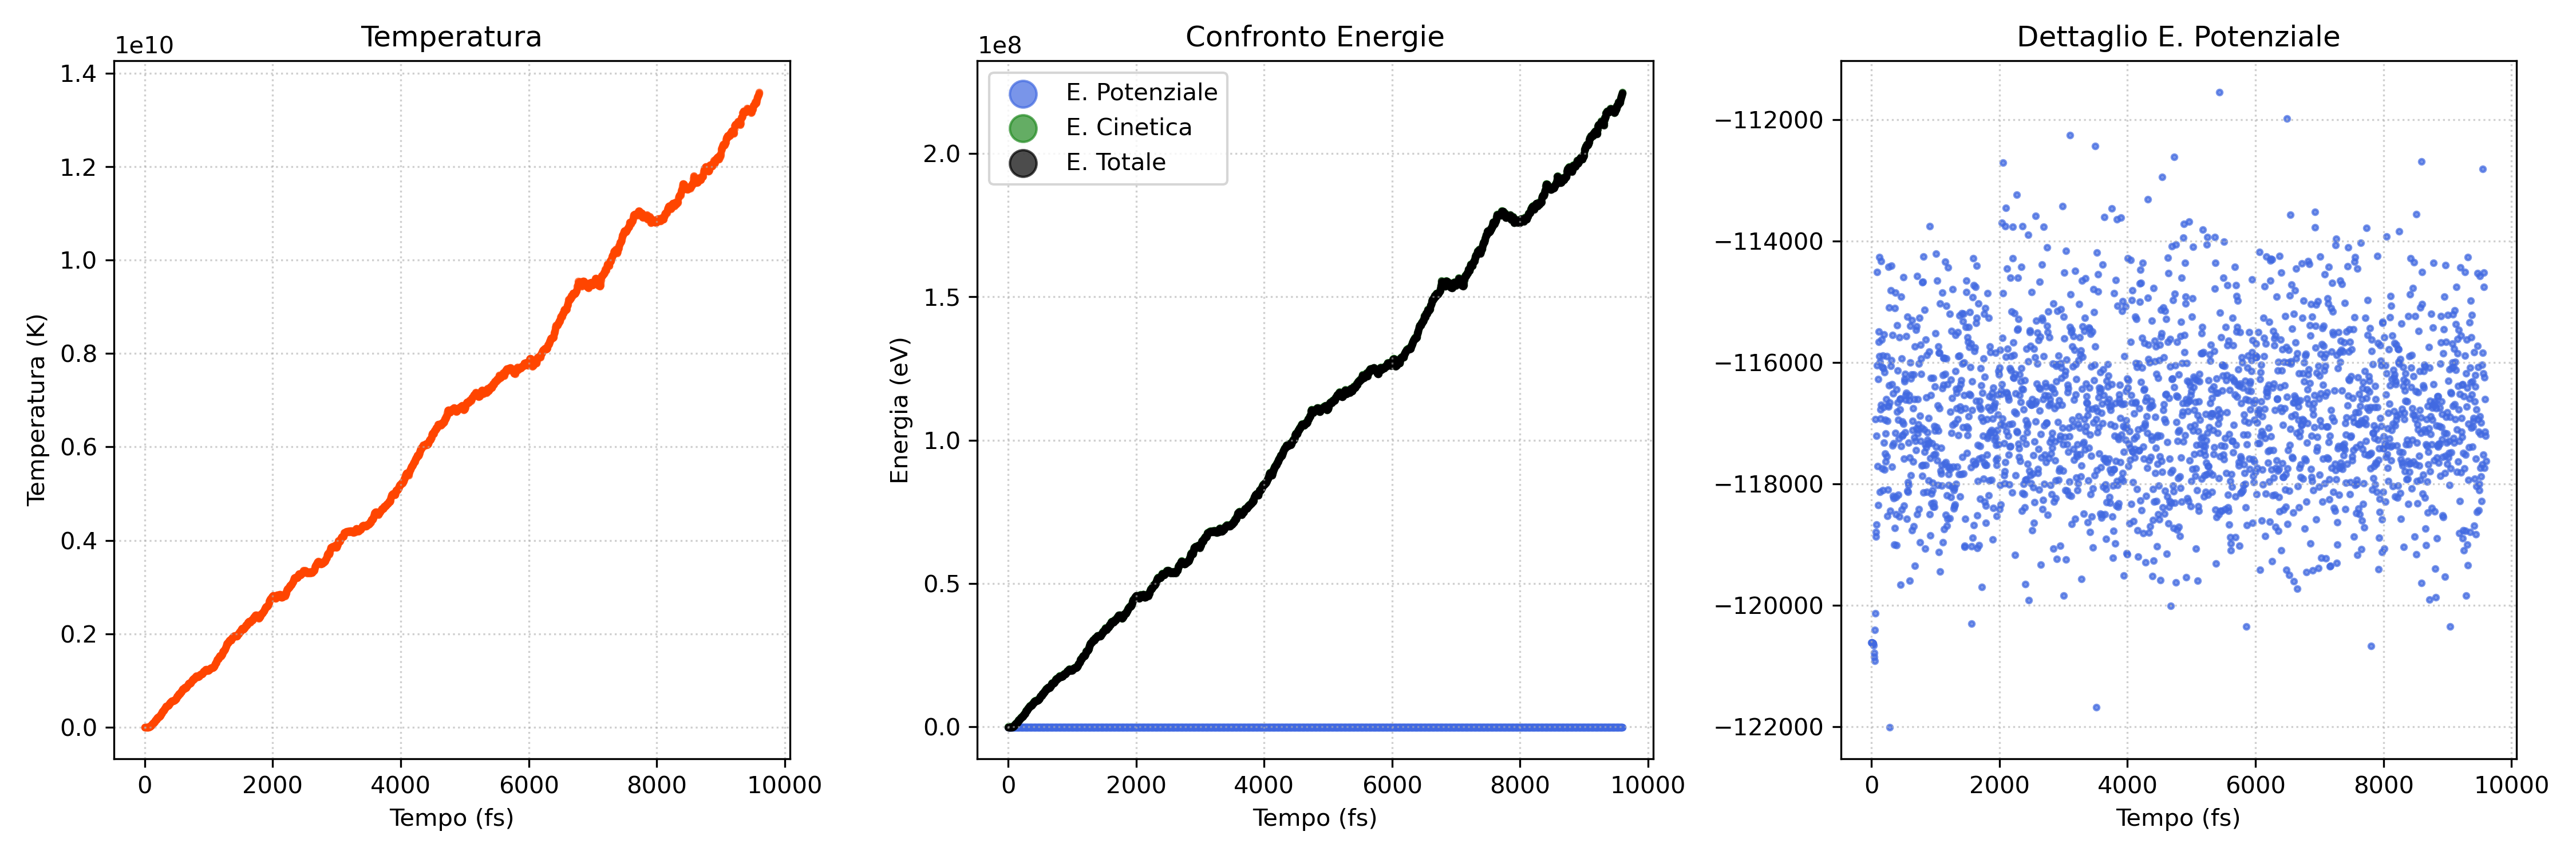
\includegraphics[scale=0.4]{./img/andamento_energia_nve_testdata.png}
    \caption{Grafico dell'andamento temporale per i valori di energia e temperatura.}
    \label{fig:andamento_nve-testdata}
\end{figure}

possiamo notare \ref{fig:andamento_nve-testdata} che i valori di energia e temperatura divergono a valori fisicamente insensati.
L'energia potenziale oscilla entro valori limite, notiamo comunque che l'intervallo di oscillazione è relativamente ampio.

Risulta utile anche guardare ai valori di forza associati a queste dinamica, riportati nel seguente grafico

\begin{figure}[h]
    \centering
    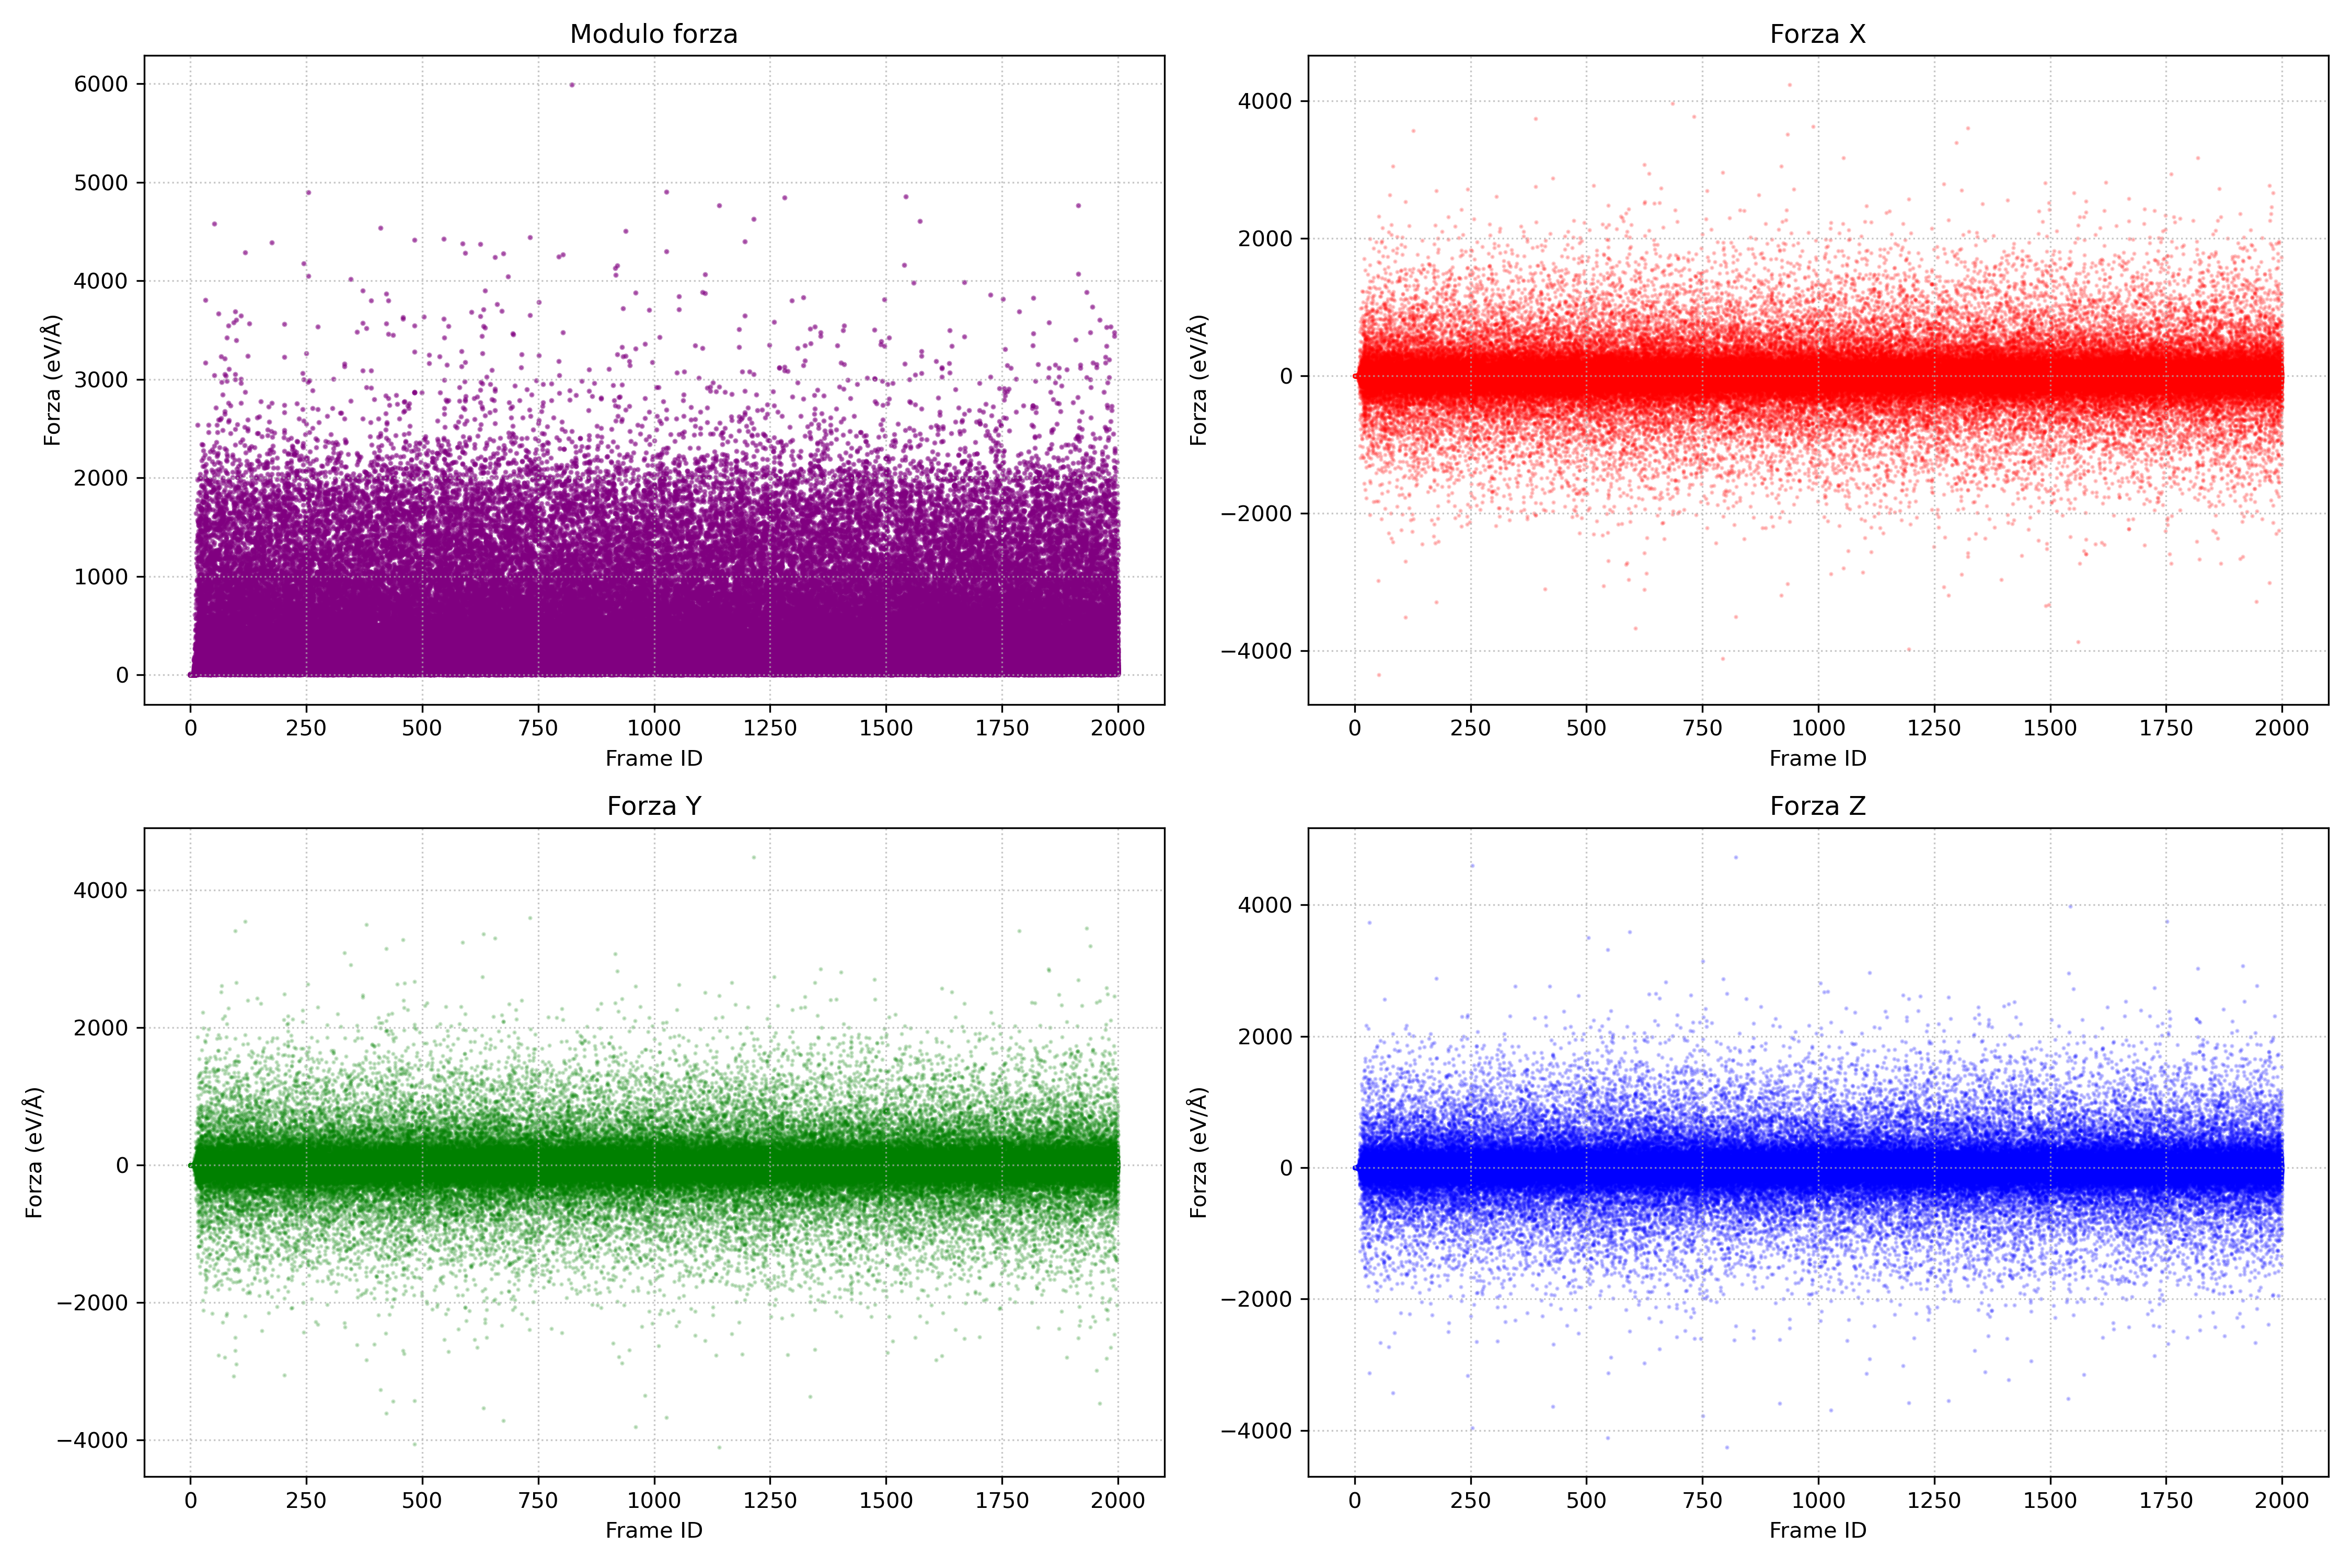
\includegraphics[scale=0.35]{./img/andamento_forze_totali_blocchi_nve_testdata.png}
    \caption{Grafico dell'andamento temporale per i valori di forza, sia in modulo che divise per componenti. }
    \label{fig:andamento_nve_forze-testdata}
\end{figure}

anche in questo caso possiamo notare che otteniamo valori estremamente elevati.



\section{Analisi delle problematiche} %--------------------------------------------------------------------------------------------------------------------------------------------------------------------------------------------------------

Abbiamo precedentemente menzionato che il potenziale è stato addestrato con parametri di soap non troppo elevati. Poniamo questo come ultimo problema da verificare in quanto i risultati sulle configurazioni di test erano discreti.
In questa sezioni ci poniamo di modificare a turno vari parametri, o combinazioni di tali, in modo da poter identificare quale sia il problema.


\subsection{Temperatura}

Come primo test abbiamo provato a modificare la temperatura dalla quale venivano estratti i valori di velocità. 
Si è impostato questo valore a $0$K, gli altri parametri sono rimasti invariati. 
Anche in questo caso diamo sia i riaultati per i valori di energia e temperatura

\begin{figure}[h]
    \centering
    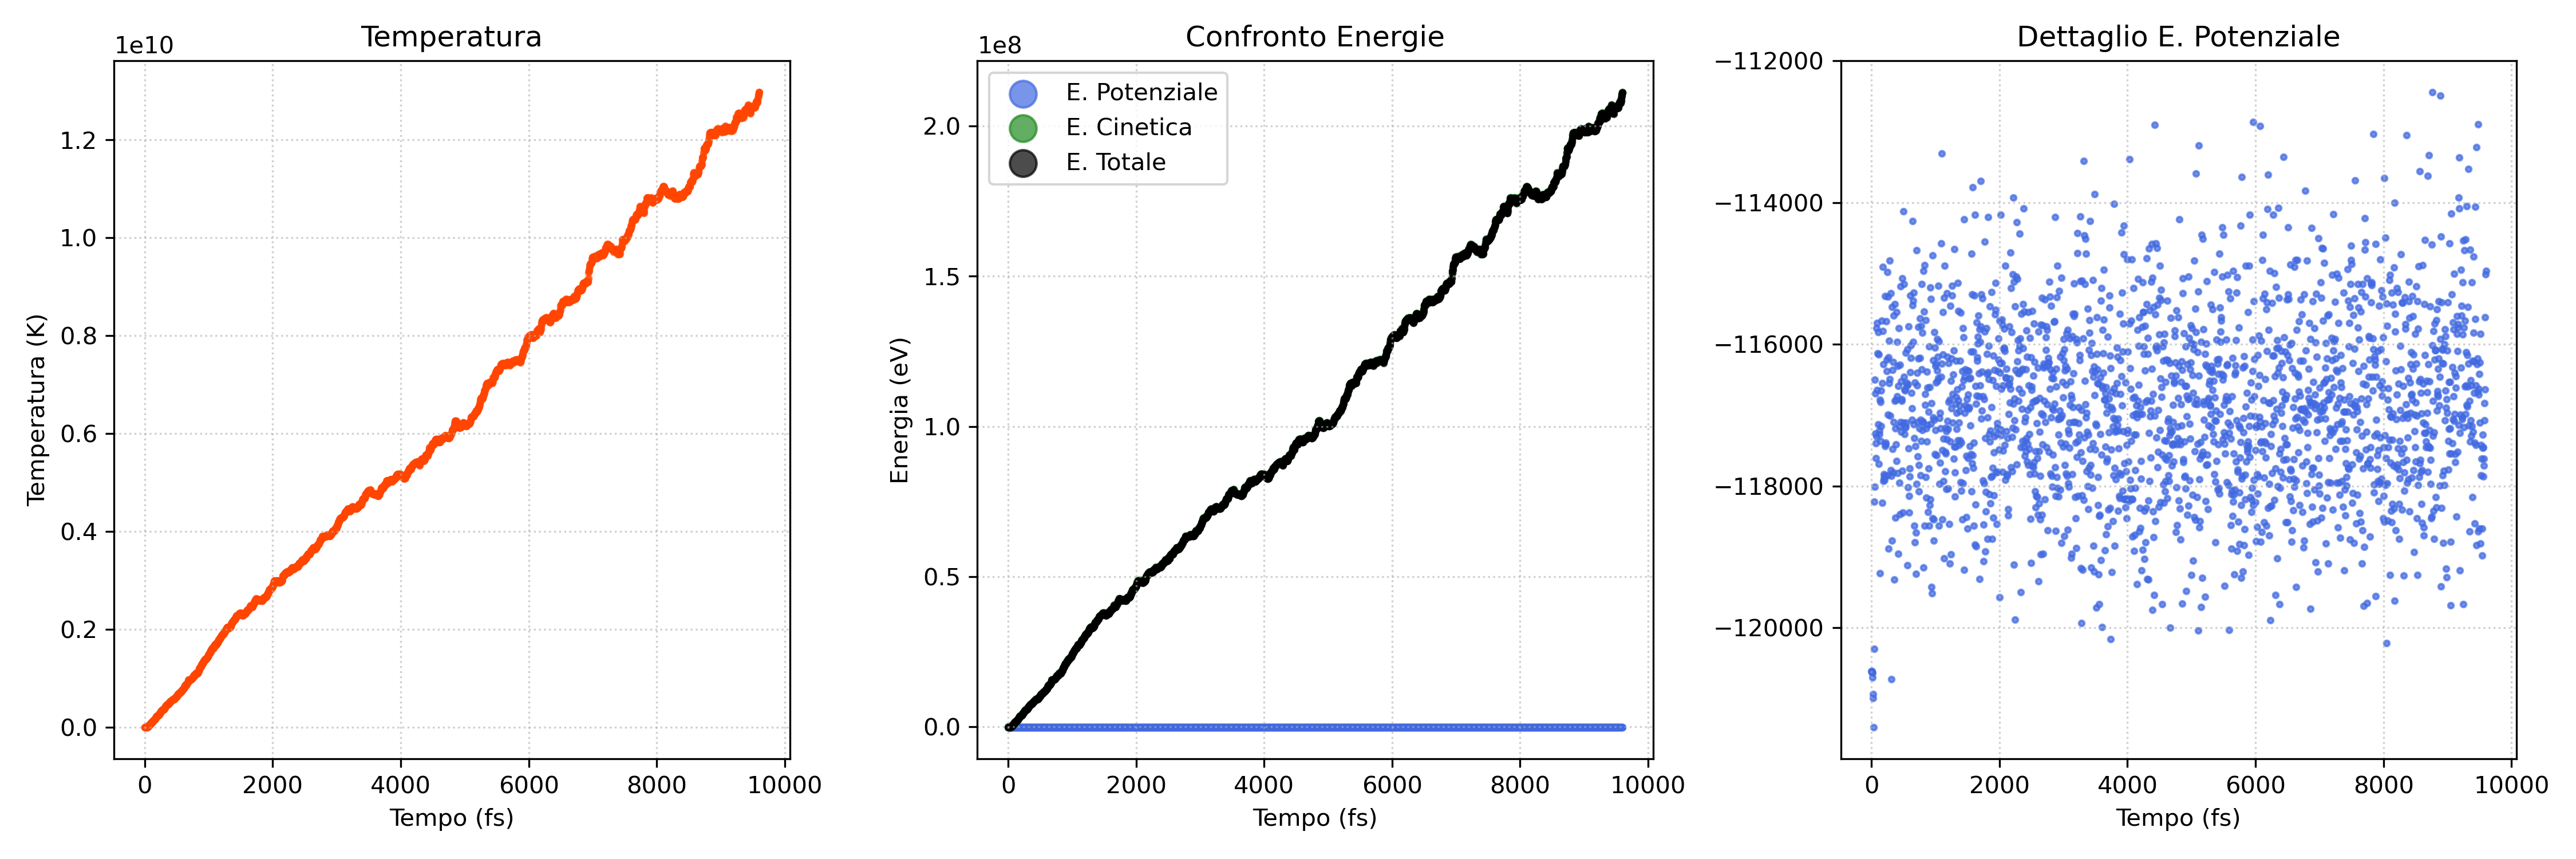
\includegraphics[scale=0.4]{./img/andamento_energia_nve_testdata_0k.png}
    \caption{Grafico dell'andamento temporale per i valori di energia e temperatura}
    \label{fig:andamento_nve-traindata_0k}
\end{figure}

che per i valori delle forze

\begin{figure}[h]
    \centering
    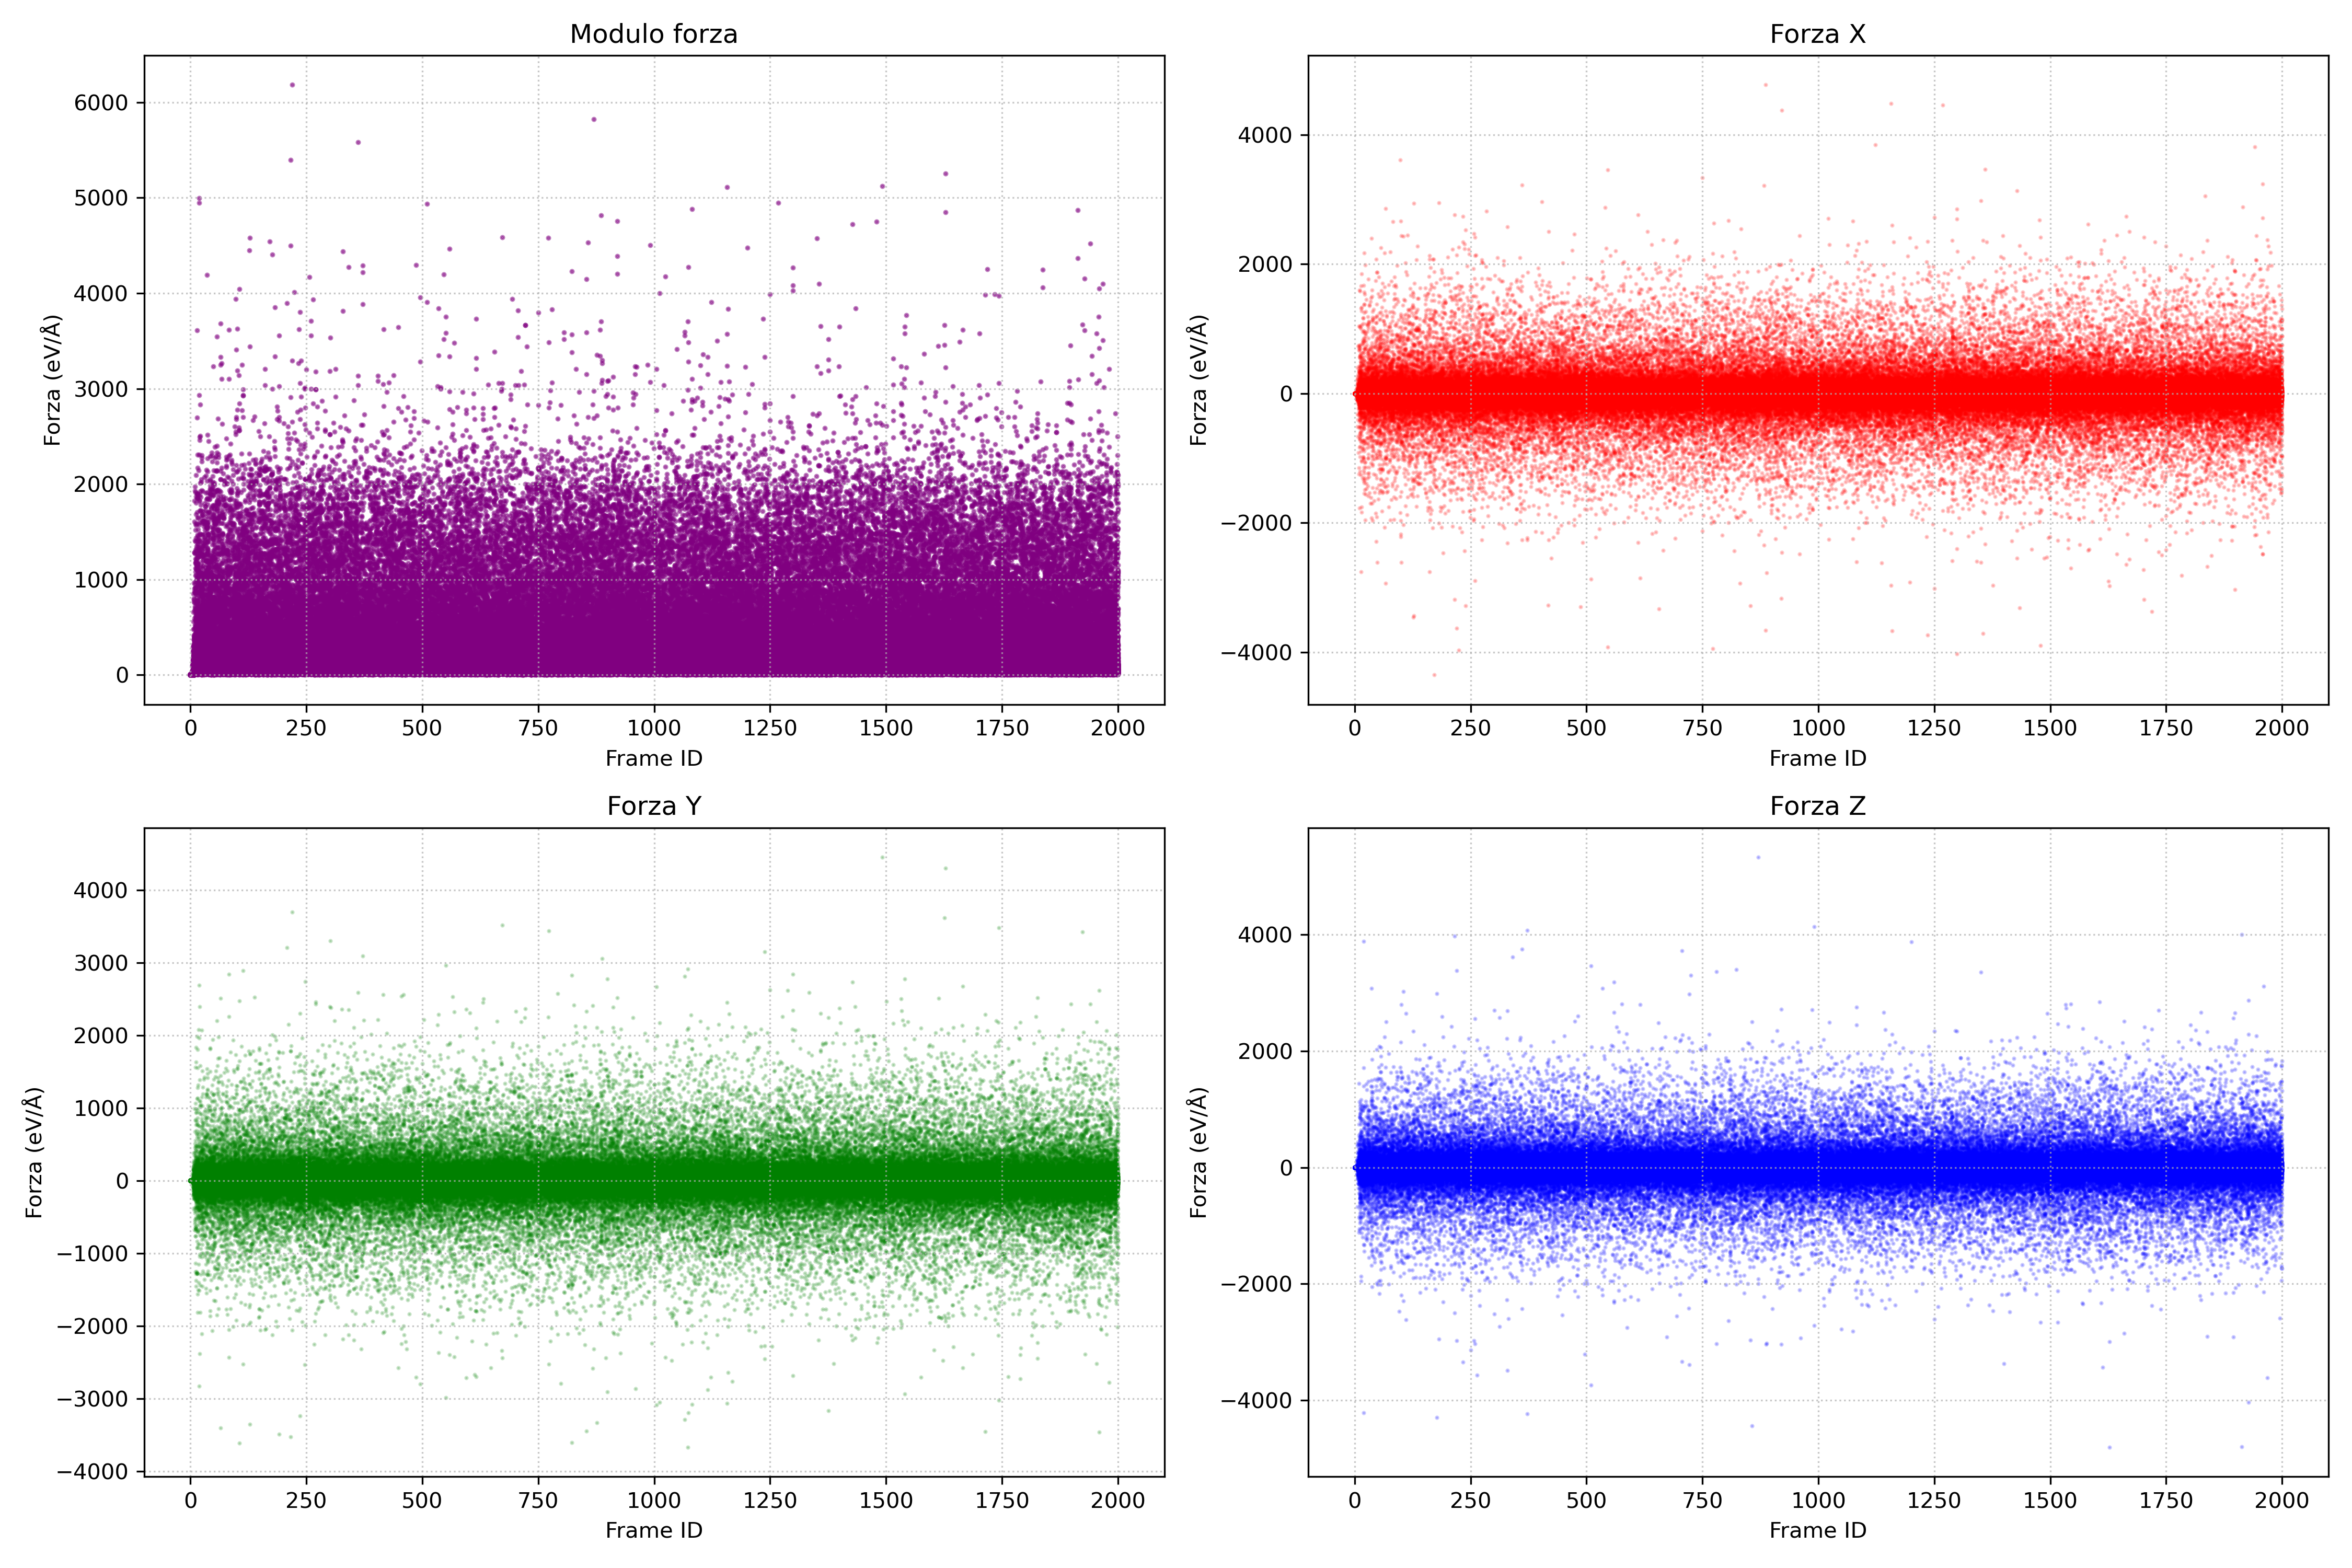
\includegraphics[scale=0.35]{./img/andamento_forze_totali_blocchi_nve_testdata_0k.png}
    \caption{Grafico dell'andamento temporale per i valori di forza, sia in modulo che divise per componenti. }
    \label{fig:andamento_nve_forze-traindata_0k}
\end{figure}

Si nota \ref{fig:andamento_nve-traindata_0k} e \ref{fig:andamento_nve_forze-traindata_0k} che il risultato non è dissimile da quello ottenuto in precedenza, possiamo quindi escludere che sia un problema legato al valore di temperatura.



\subsection{Timestep} %----------------------------------------------------------------------------------------------------------------------------------------------------------------------------------------------------------------------

Per questa analisi sono stati provati diversi valori di timestep, riportiamo solo uno di questi.
Come timestep si è impostato un valori di $10^{-5}$fs, e un totale di $50'000$ iterazioni, in modo da valutate la stabilità sul lungo periodo. Si è mantenuta una temperatura di $3'000$K.

I valori di energia e temperatura sono rappresentati nel seguente grafico \ref{fig:andamento_nve_energie_timestep}

\begin{figure}[h]
    \centering
    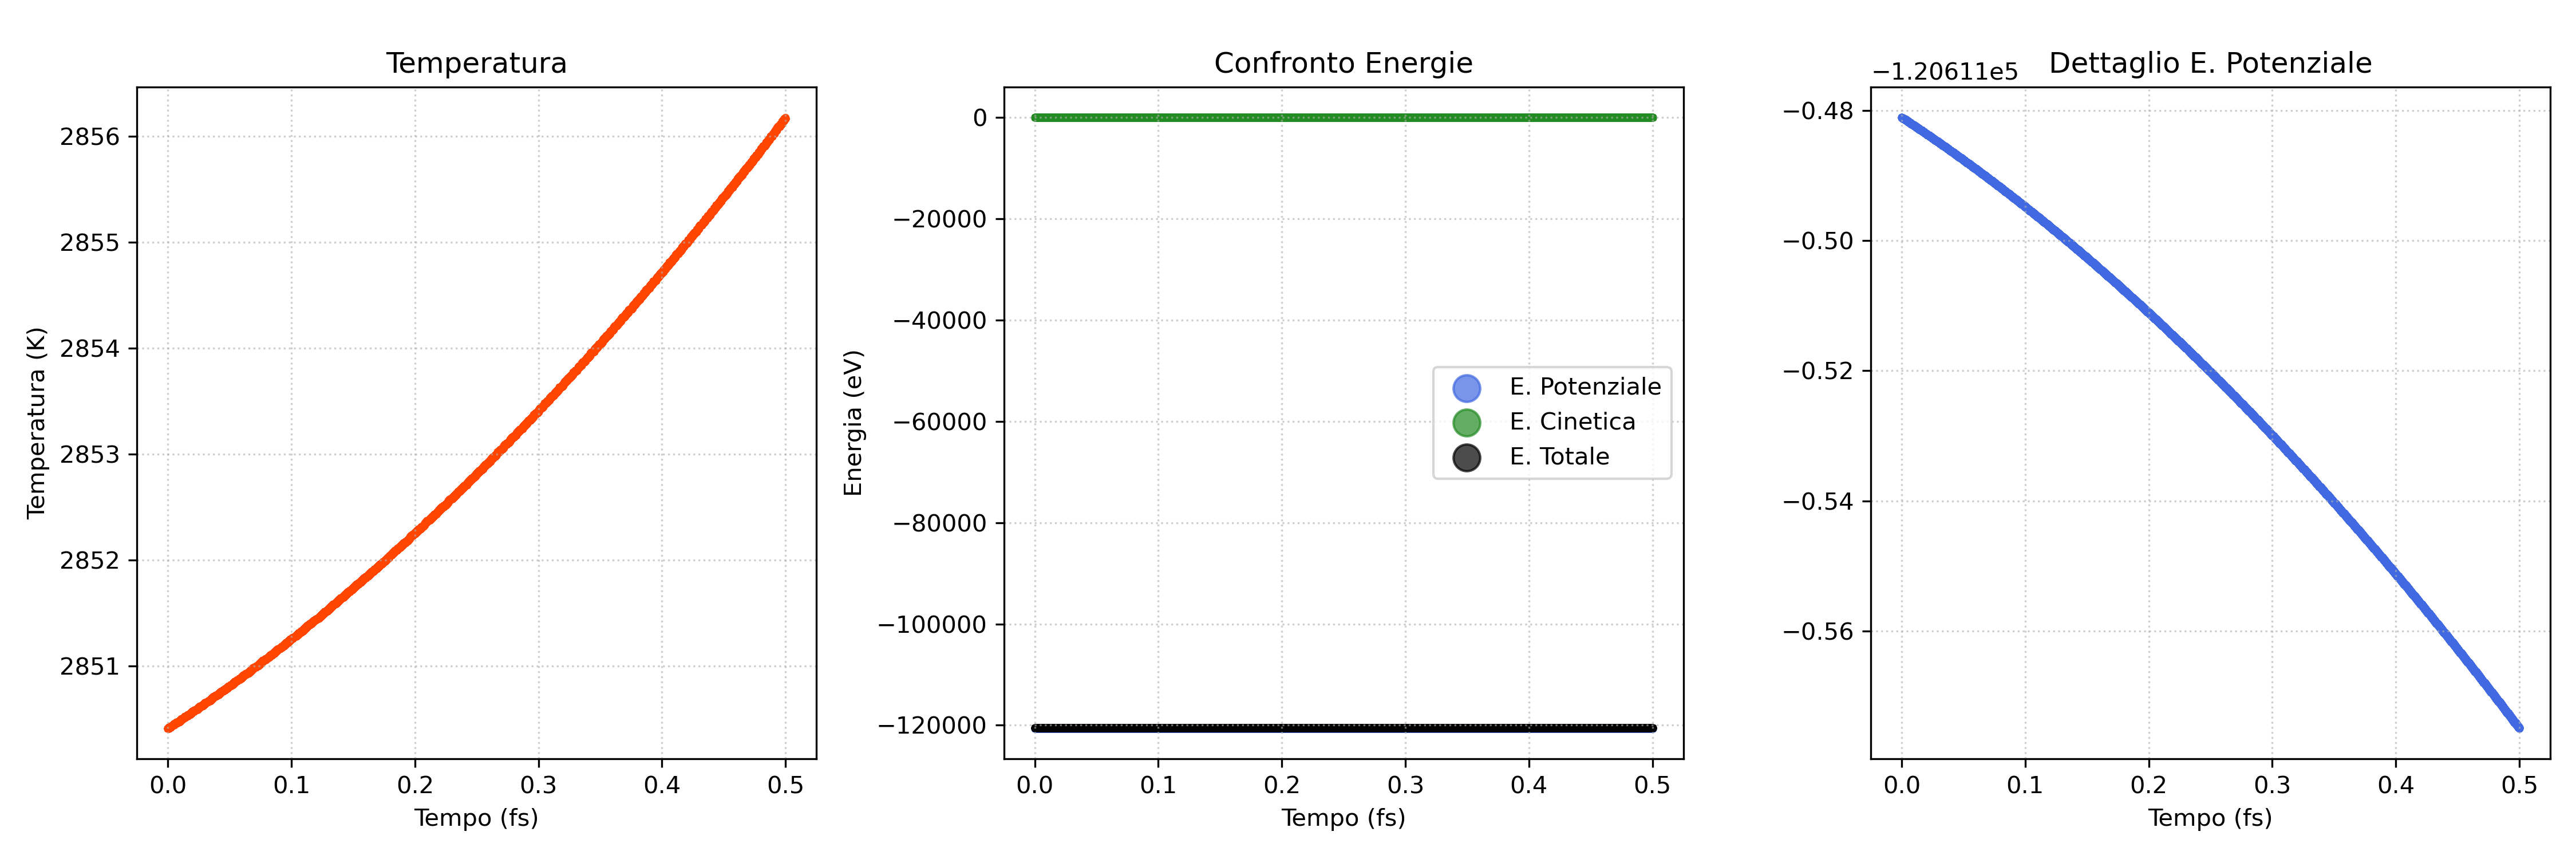
\includegraphics[scale=0.4]{./img/andamento_energia_nve_timestep.png}
    \caption{Grafico dell'andamento temporale per i valori di energia e temperatura}
    \label{fig:andamento_nve_energie_timestep}
\end{figure}

mentre per quanto riguarda le forze otteniamo il grafico \ref{fig:andamento_nve_forze_timestep}


\begin{figure}[h]
    \centering
    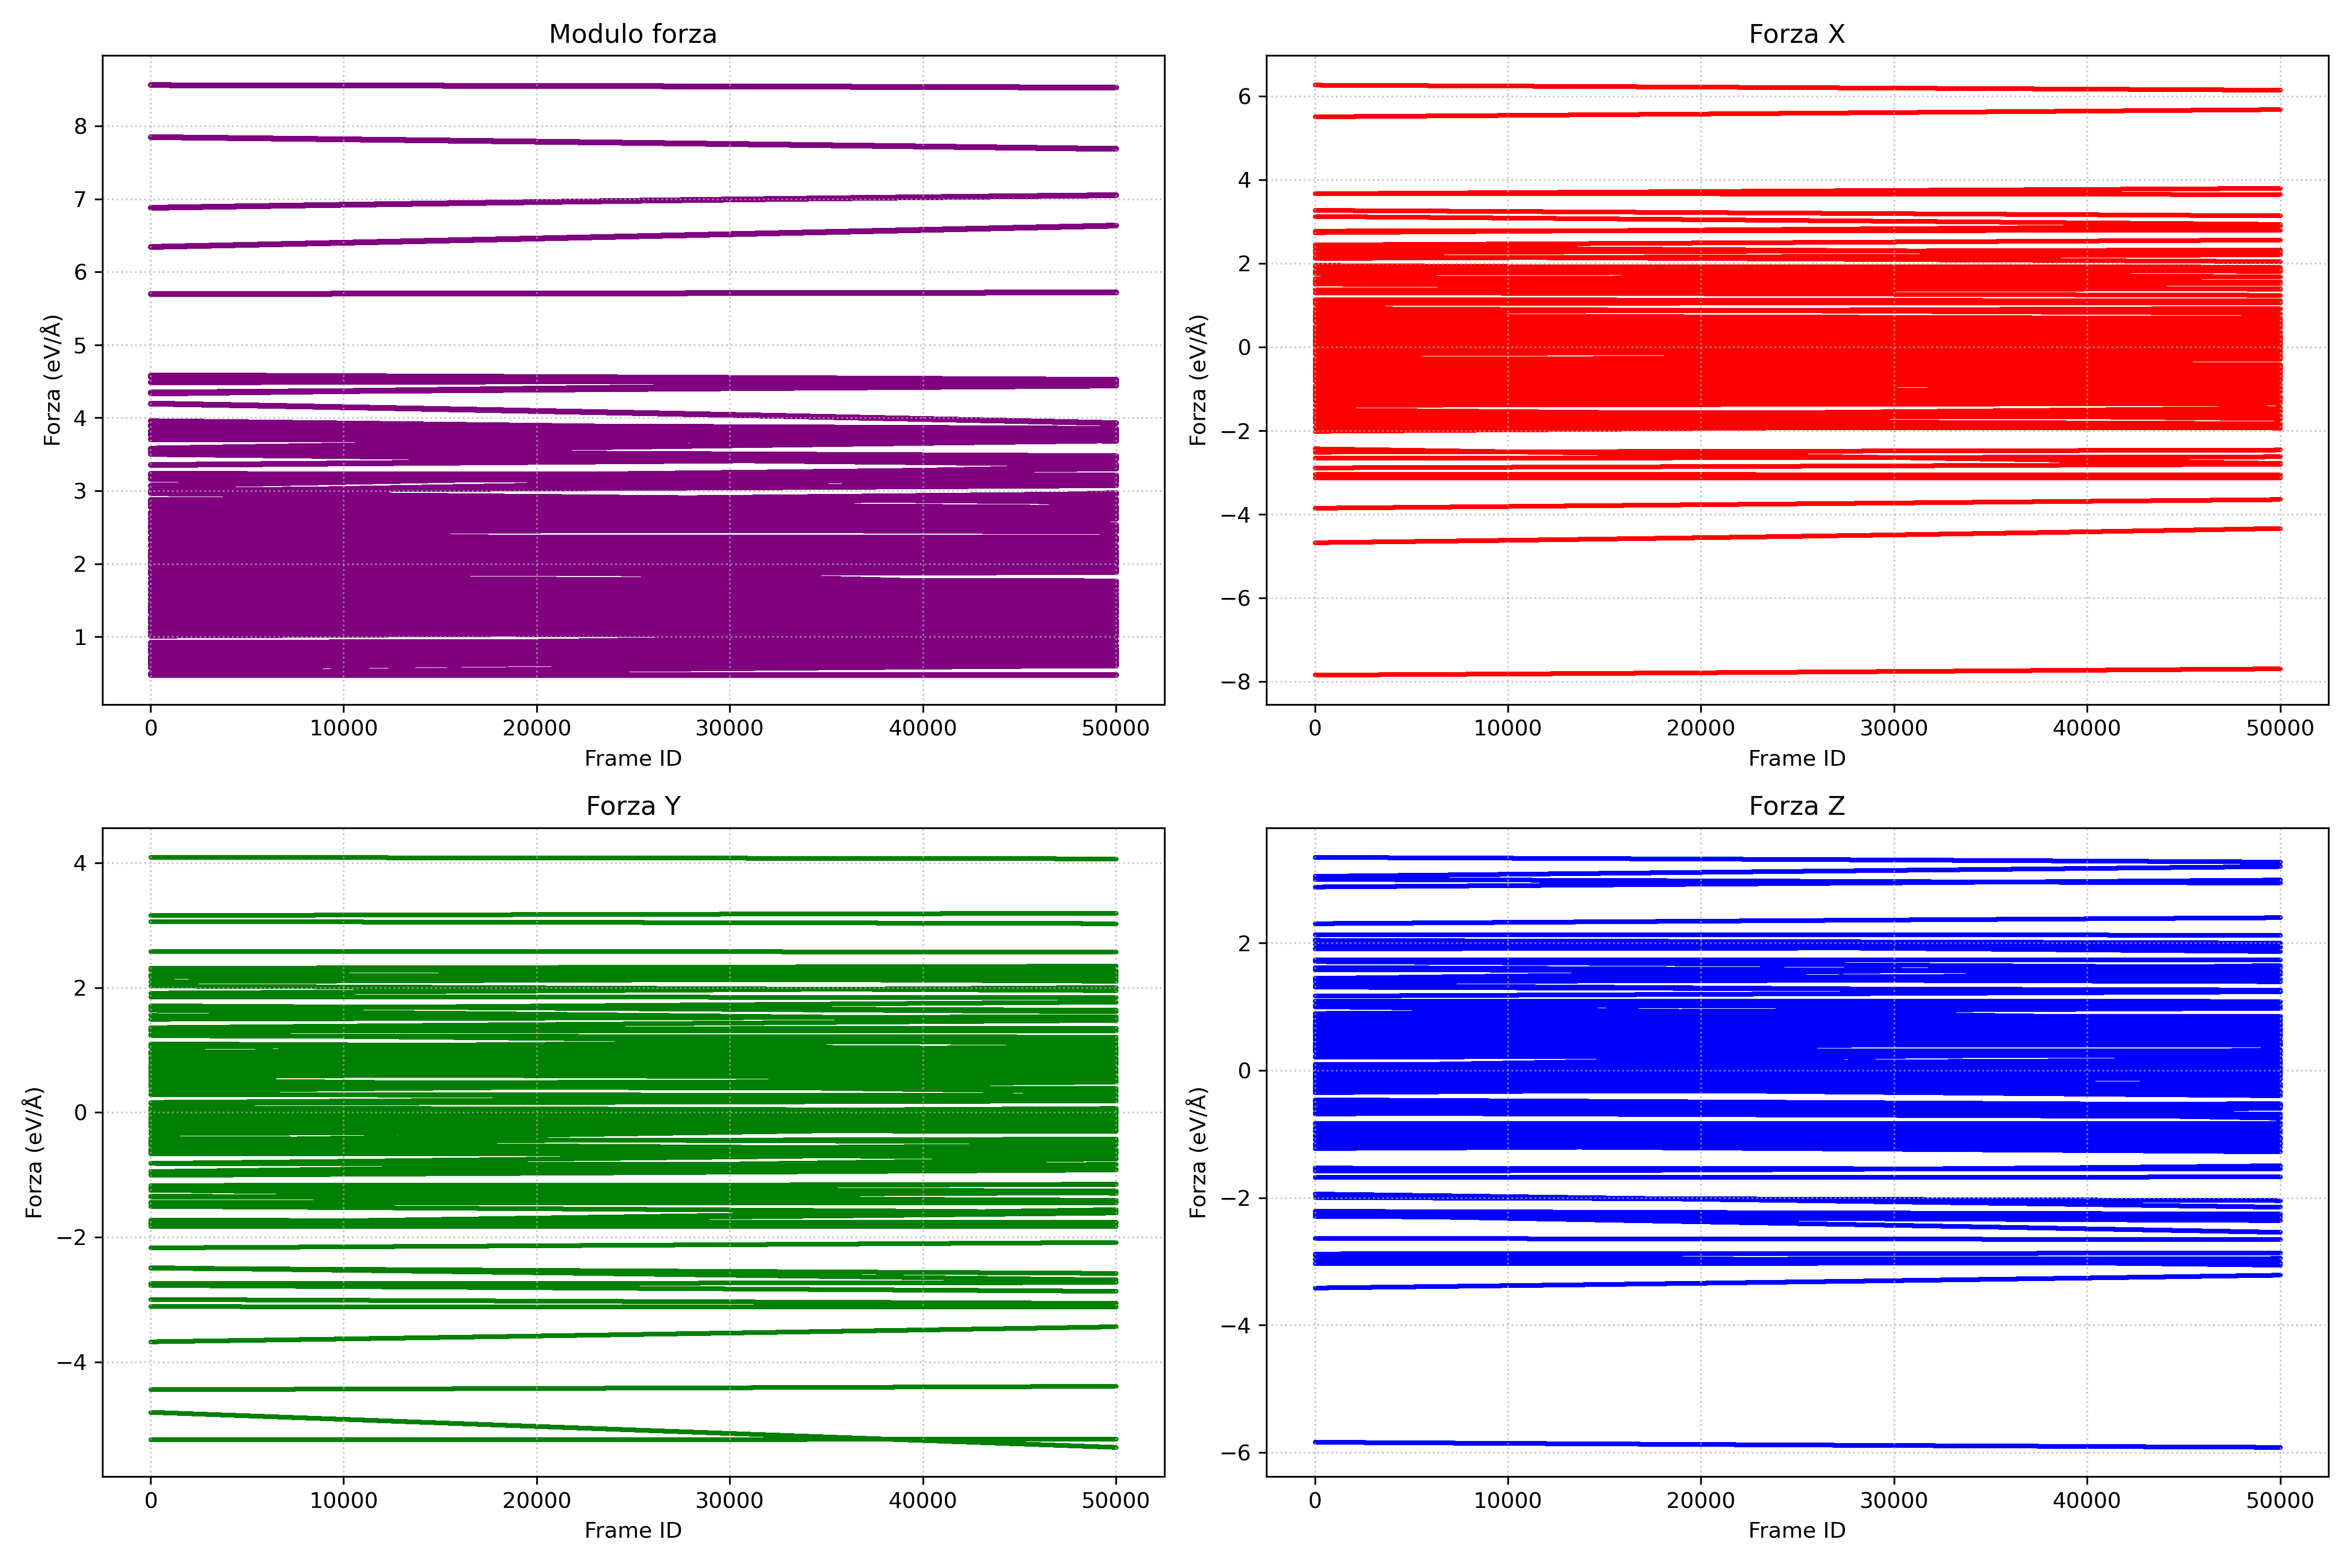
\includegraphics[scale=0.35]{./img/andamento_forze_totali_blocchi_nve_timestep.png}
    \caption{Grafico dell'andamento temporale per i valori di energia e temperatura}
    \label{fig:andamento_nve_forze_timestep}
\end{figure}


considerando questo risultato \ref{fig:andamento_nve_energie_timestep} la prima cosa che si vede è una diminuzione del range in cui i valori di temperatura e di energia variano.
Ad ogni modo possiamo notare che entrambe mantengono la medesima forma vista in precedenza, possiamo quindi presumere che stiano comunque divergendo, ma ad un rate estremamente basso.
Anche i valori delle forze sono contenuti.
Considerando la tipologia di integratore numerico utilizzato in questa simulazione, questo risultato era prevedibile.


\subsection{Distanze e forze}

Risulta utile andare a guardare la distribuzione dei valori delle distanze tra i primi vicini, per ogni frame si prente come atomo il $j$-esimo e se ne calcola la distanza con i restanti 125, se ne prende poi il minimo, questo per ogni atomo presente nel frame. Successivamente guardiamo la relazione tra i valori di distanza e i valori di forza.

Nei grafici a due pannelli successivi vogliamo evidenziare queste relazioni.

Per il caso del semplice potenziale GAP, come notiamo nella figura (\ref{fig:confronto_forze_distanze_gap_testdata})

{
\begin{figure}[ht]
    \centering

    \begin{subfigure}{0.48\textwidth}
        \centering
        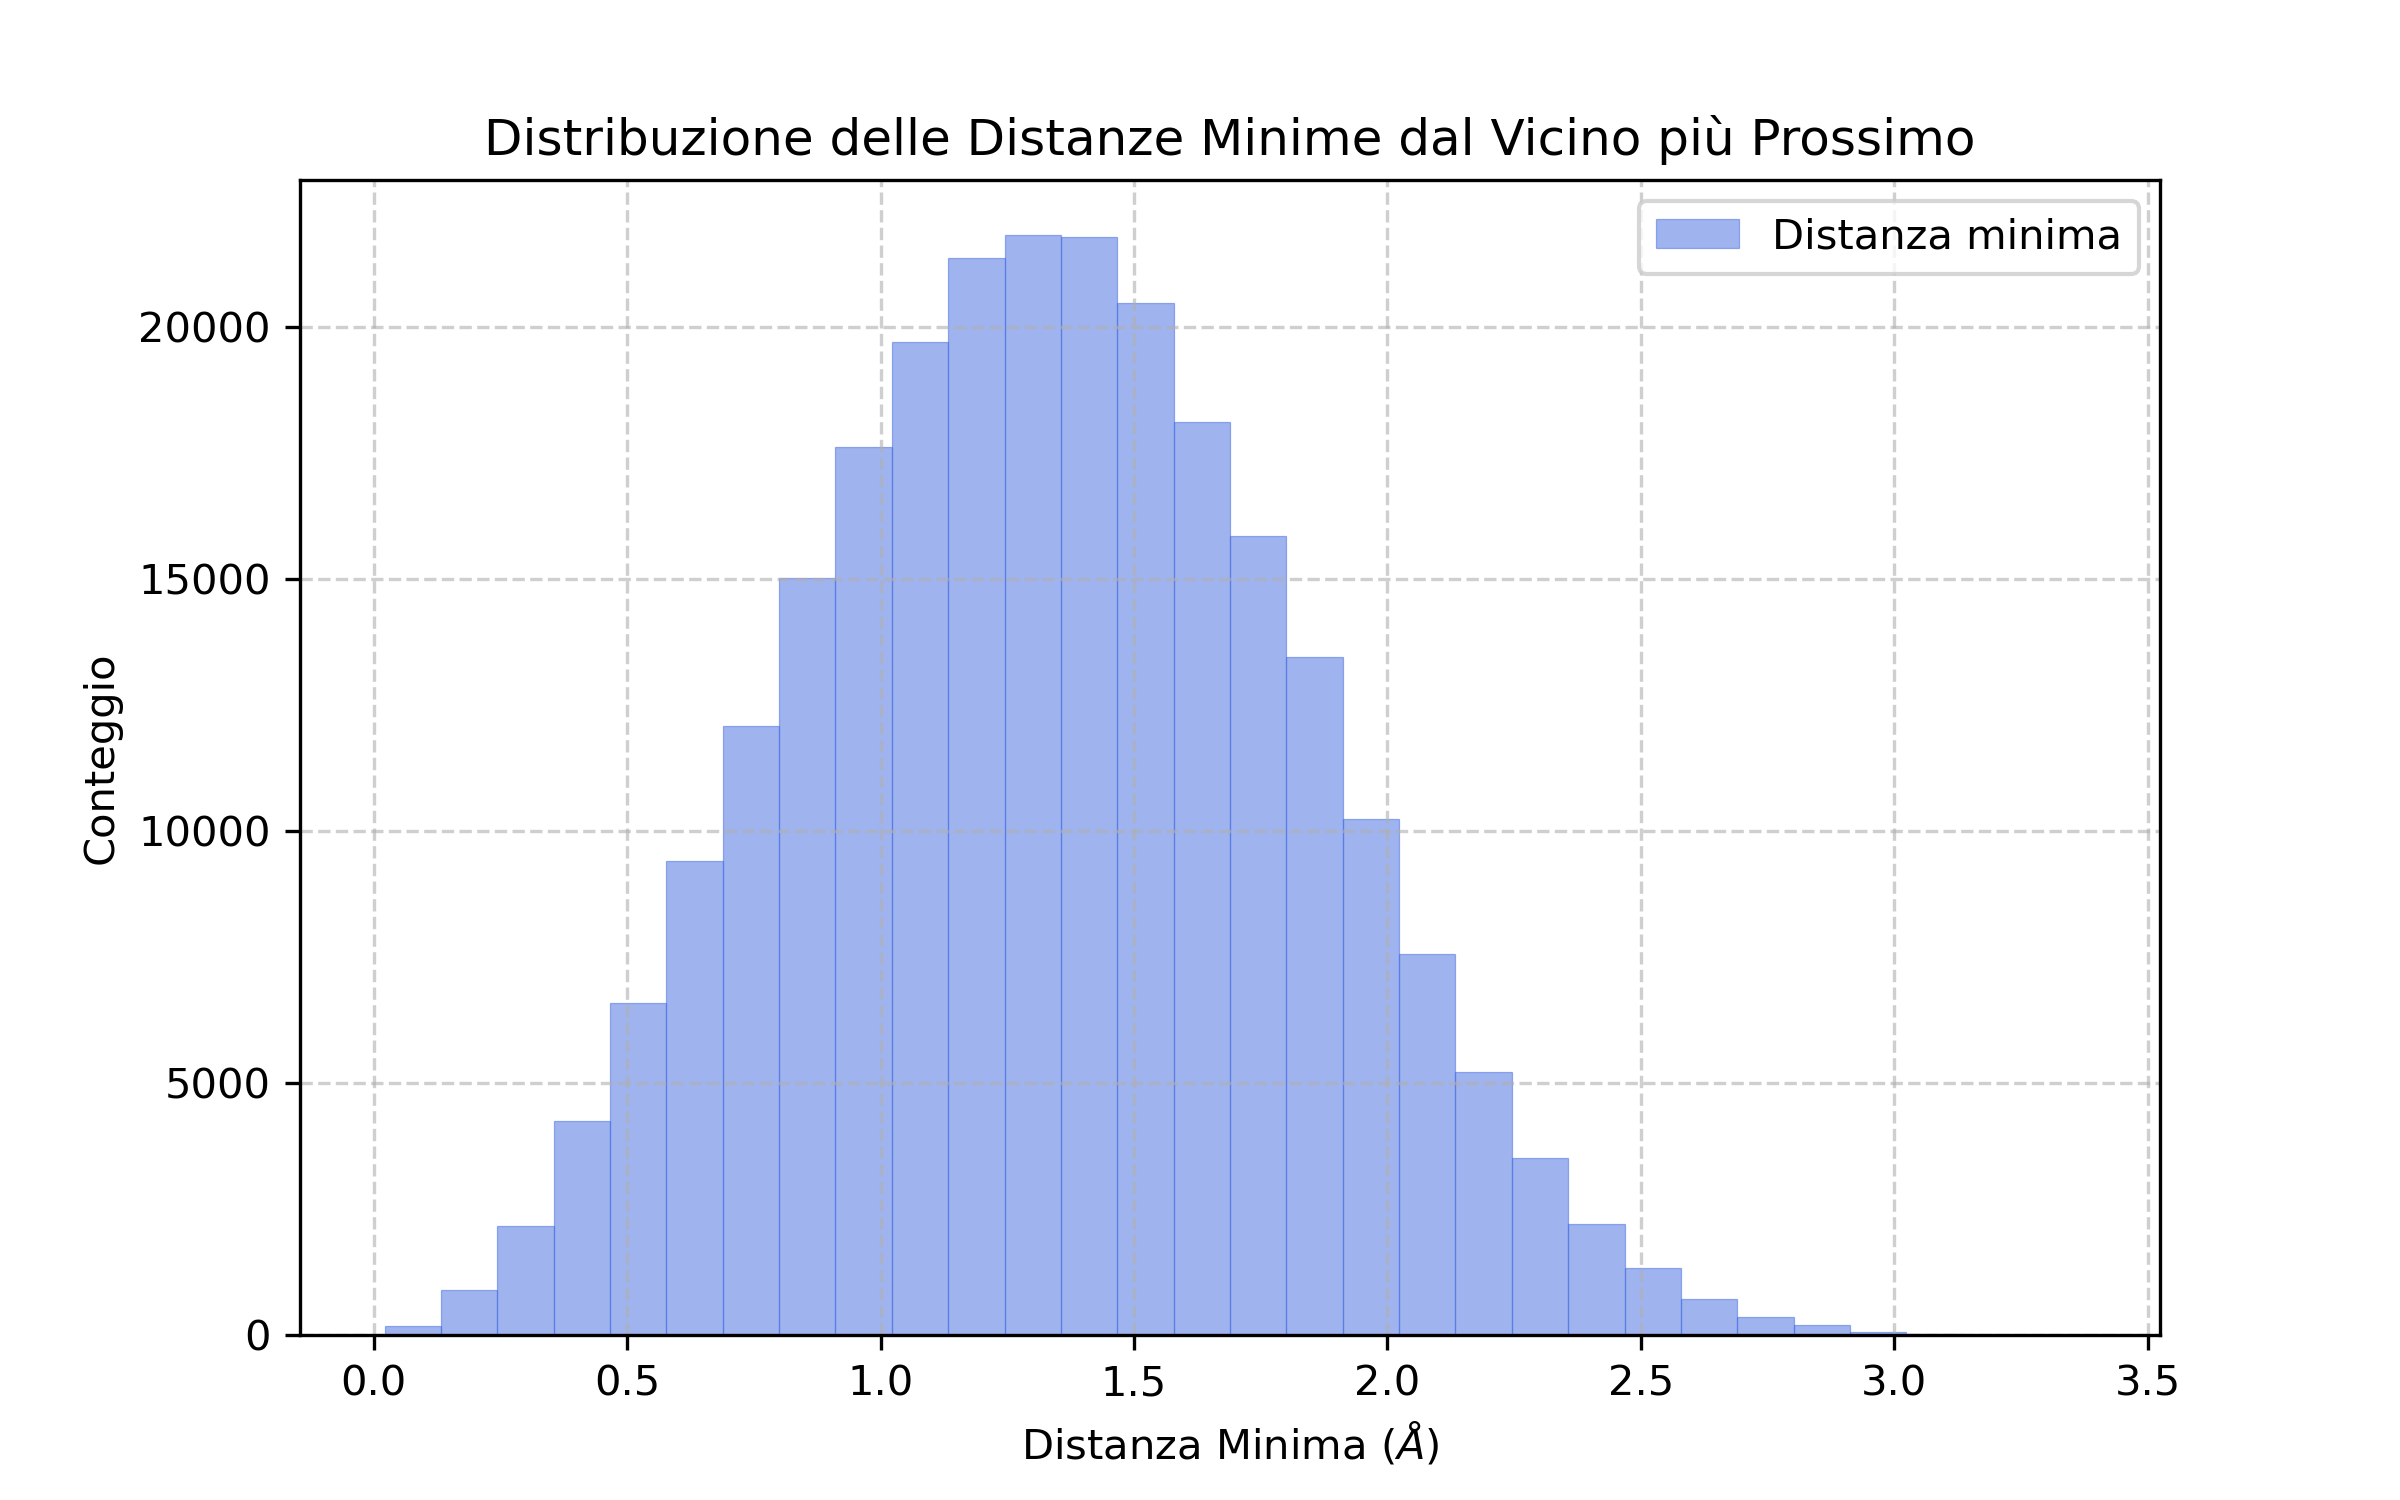
\includegraphics[width=\linewidth]{./img/histo_distanze_nve_testdata.png}
        \caption{Istogramma dei valori di distanza tra i primi vicini per il solo potenziale GAP}
    \end{subfigure}
    \hfill
    \begin{subfigure}{0.48\textwidth}
        \centering
        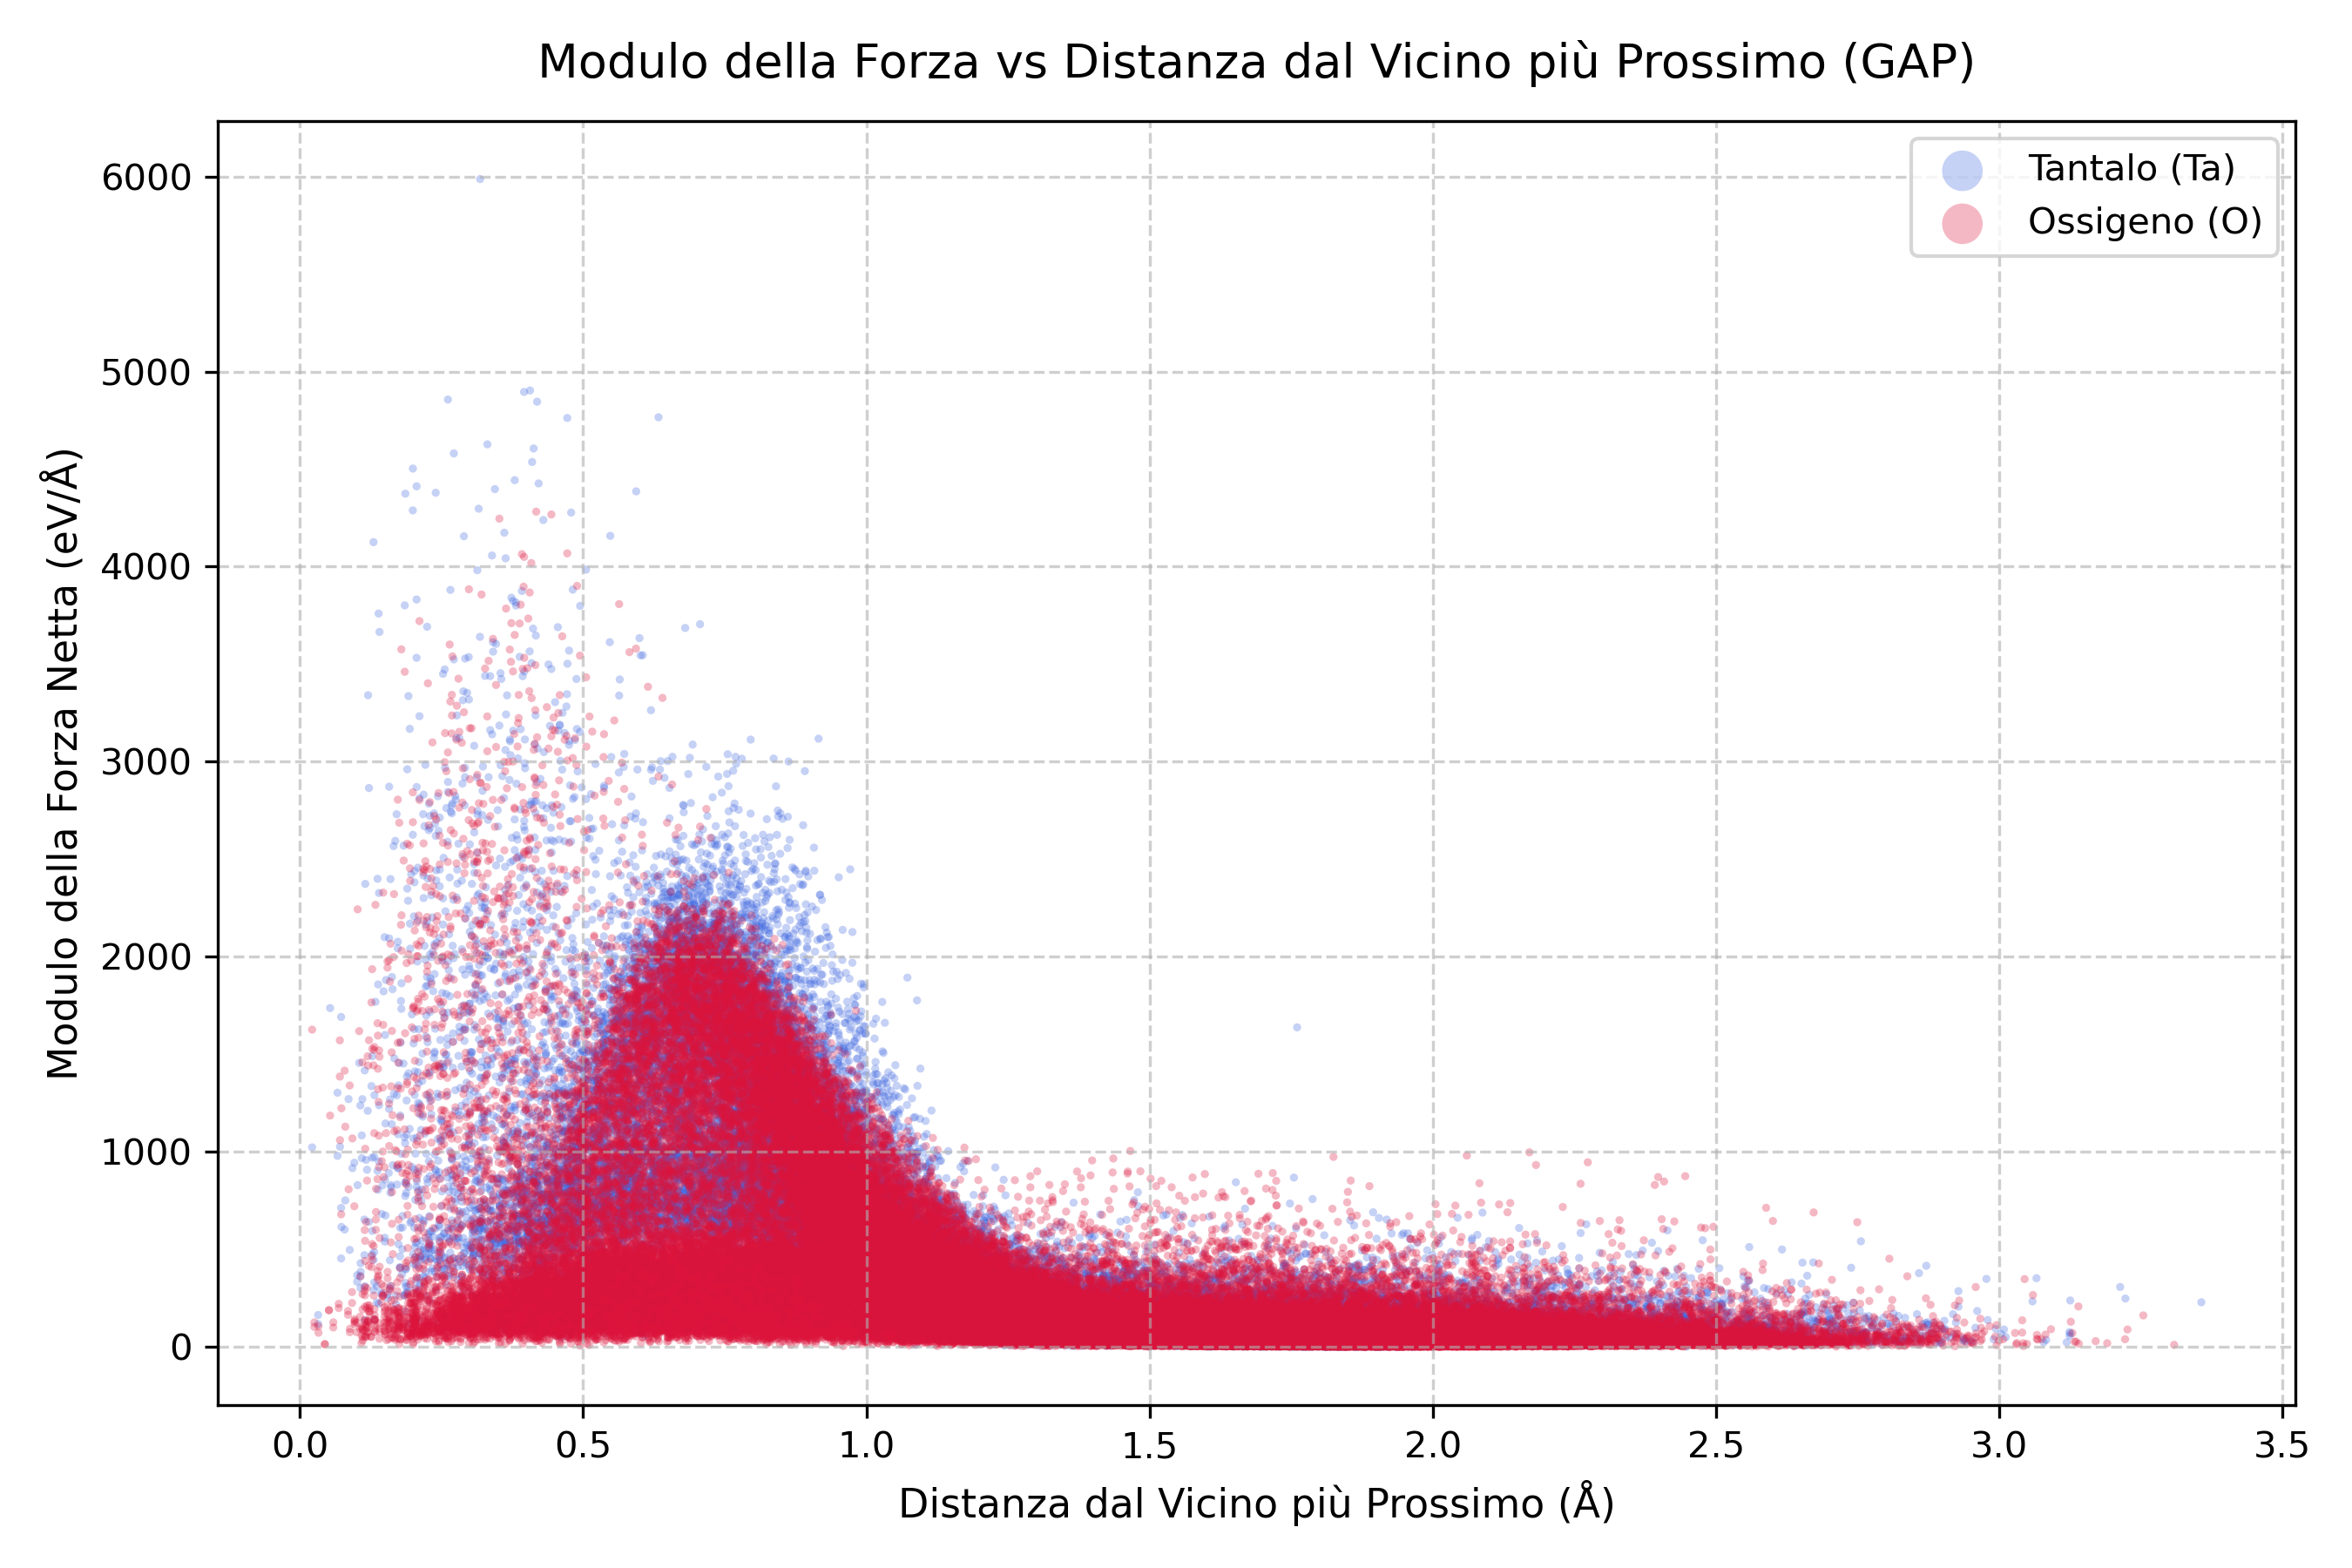
\includegraphics[width=\linewidth]{./img/andamento_forze_totali_distanza_nve_testdata.png}
        \caption{Relazione tra i valori di forza e distanza tra i primi vicini}
    \end{subfigure}

    \caption{Distanze e relazione forze distanze per il caso del solo potenziale GAP}
    \label{fig:confronto_forze_distanze_gap_testdata}
\end{figure}
}

la maggior parte dei valori di distanza si trova al di sotto del valore di $1.5$\AA. 
Si vede facilmente dove le forze assumono il loro valore maggiore.

Questo diventa rilevante nel momento in cui andiamo ad analizzare i valori di distanza tra i primi vicini e le relative forze, calcolati nel medesimo modo, presenti nelle configurazioni utilizzate nella fase di training, queste sono riportate in figura (\ref{fig:confronto_forze_distanze_qe_traindata})

{
\begin{figure}[ht]
    \centering

    \begin{subfigure}{0.48\textwidth}
        \centering
        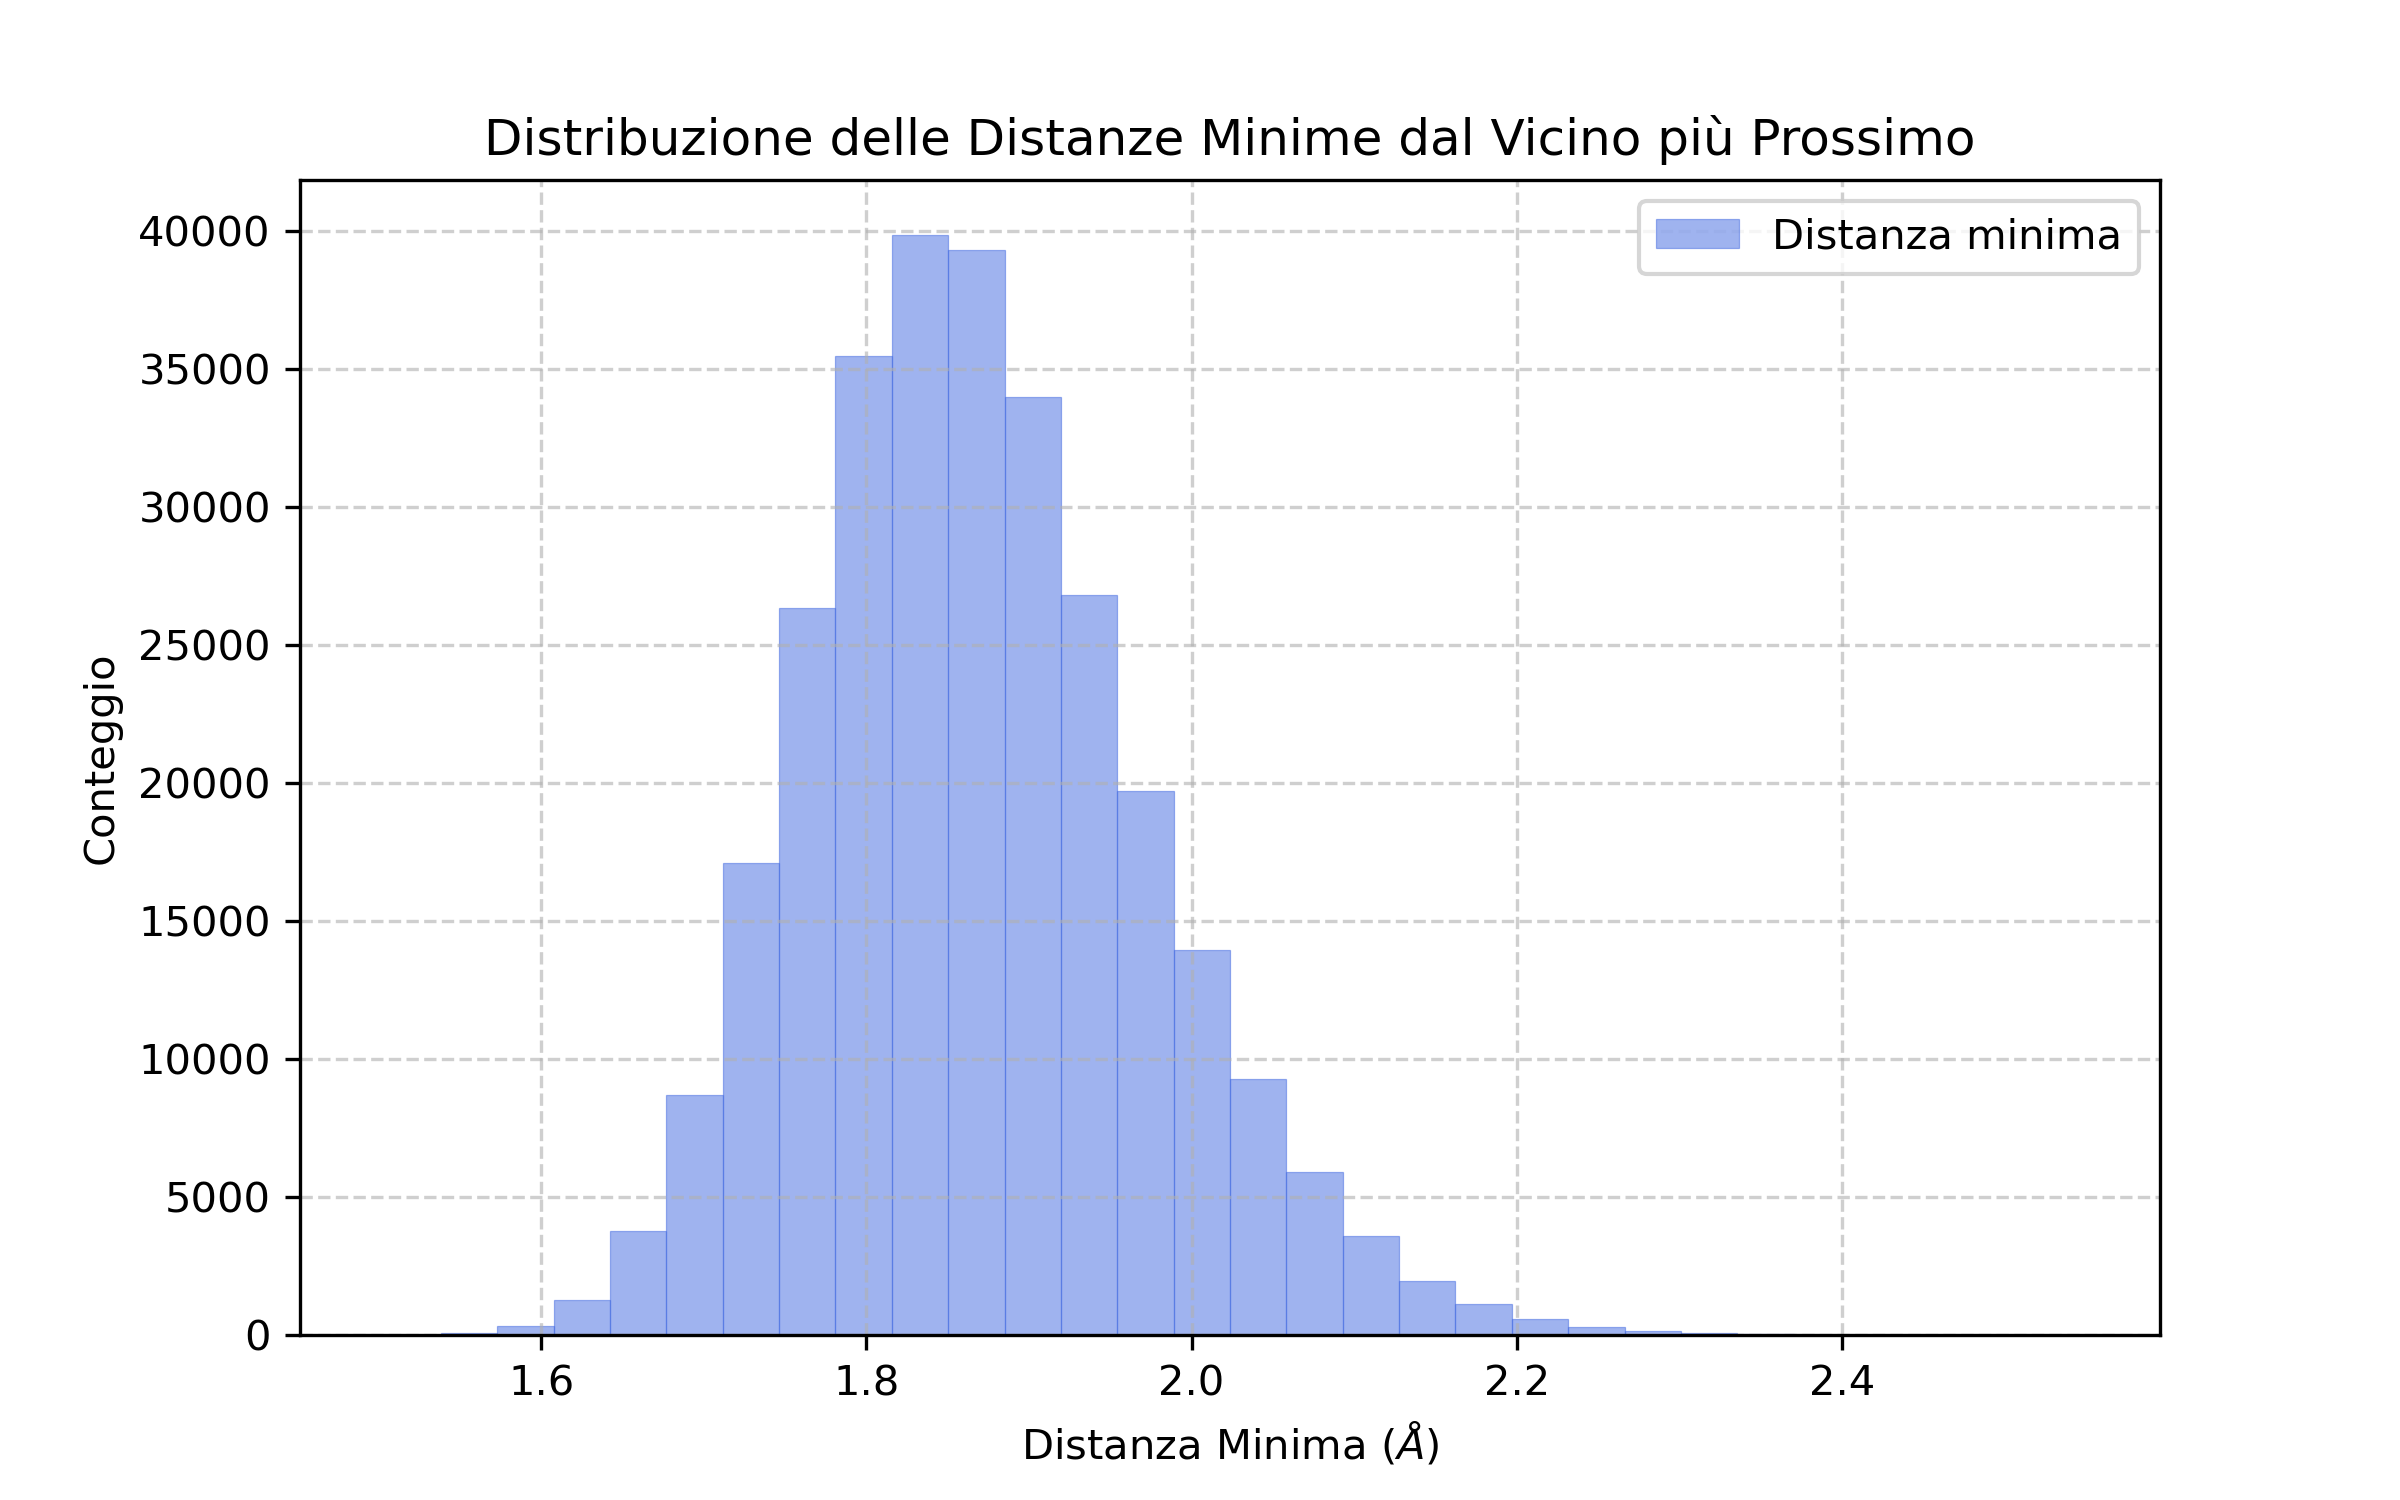
\includegraphics[width=\linewidth]{./img/histo_distanze_qe_traindata.png}
        \caption{Istogramma dei valori di distanza tra i primi vicini per il set di dati di training}
    \end{subfigure}
    \hfill
    \begin{subfigure}{0.48\textwidth}
        \centering
        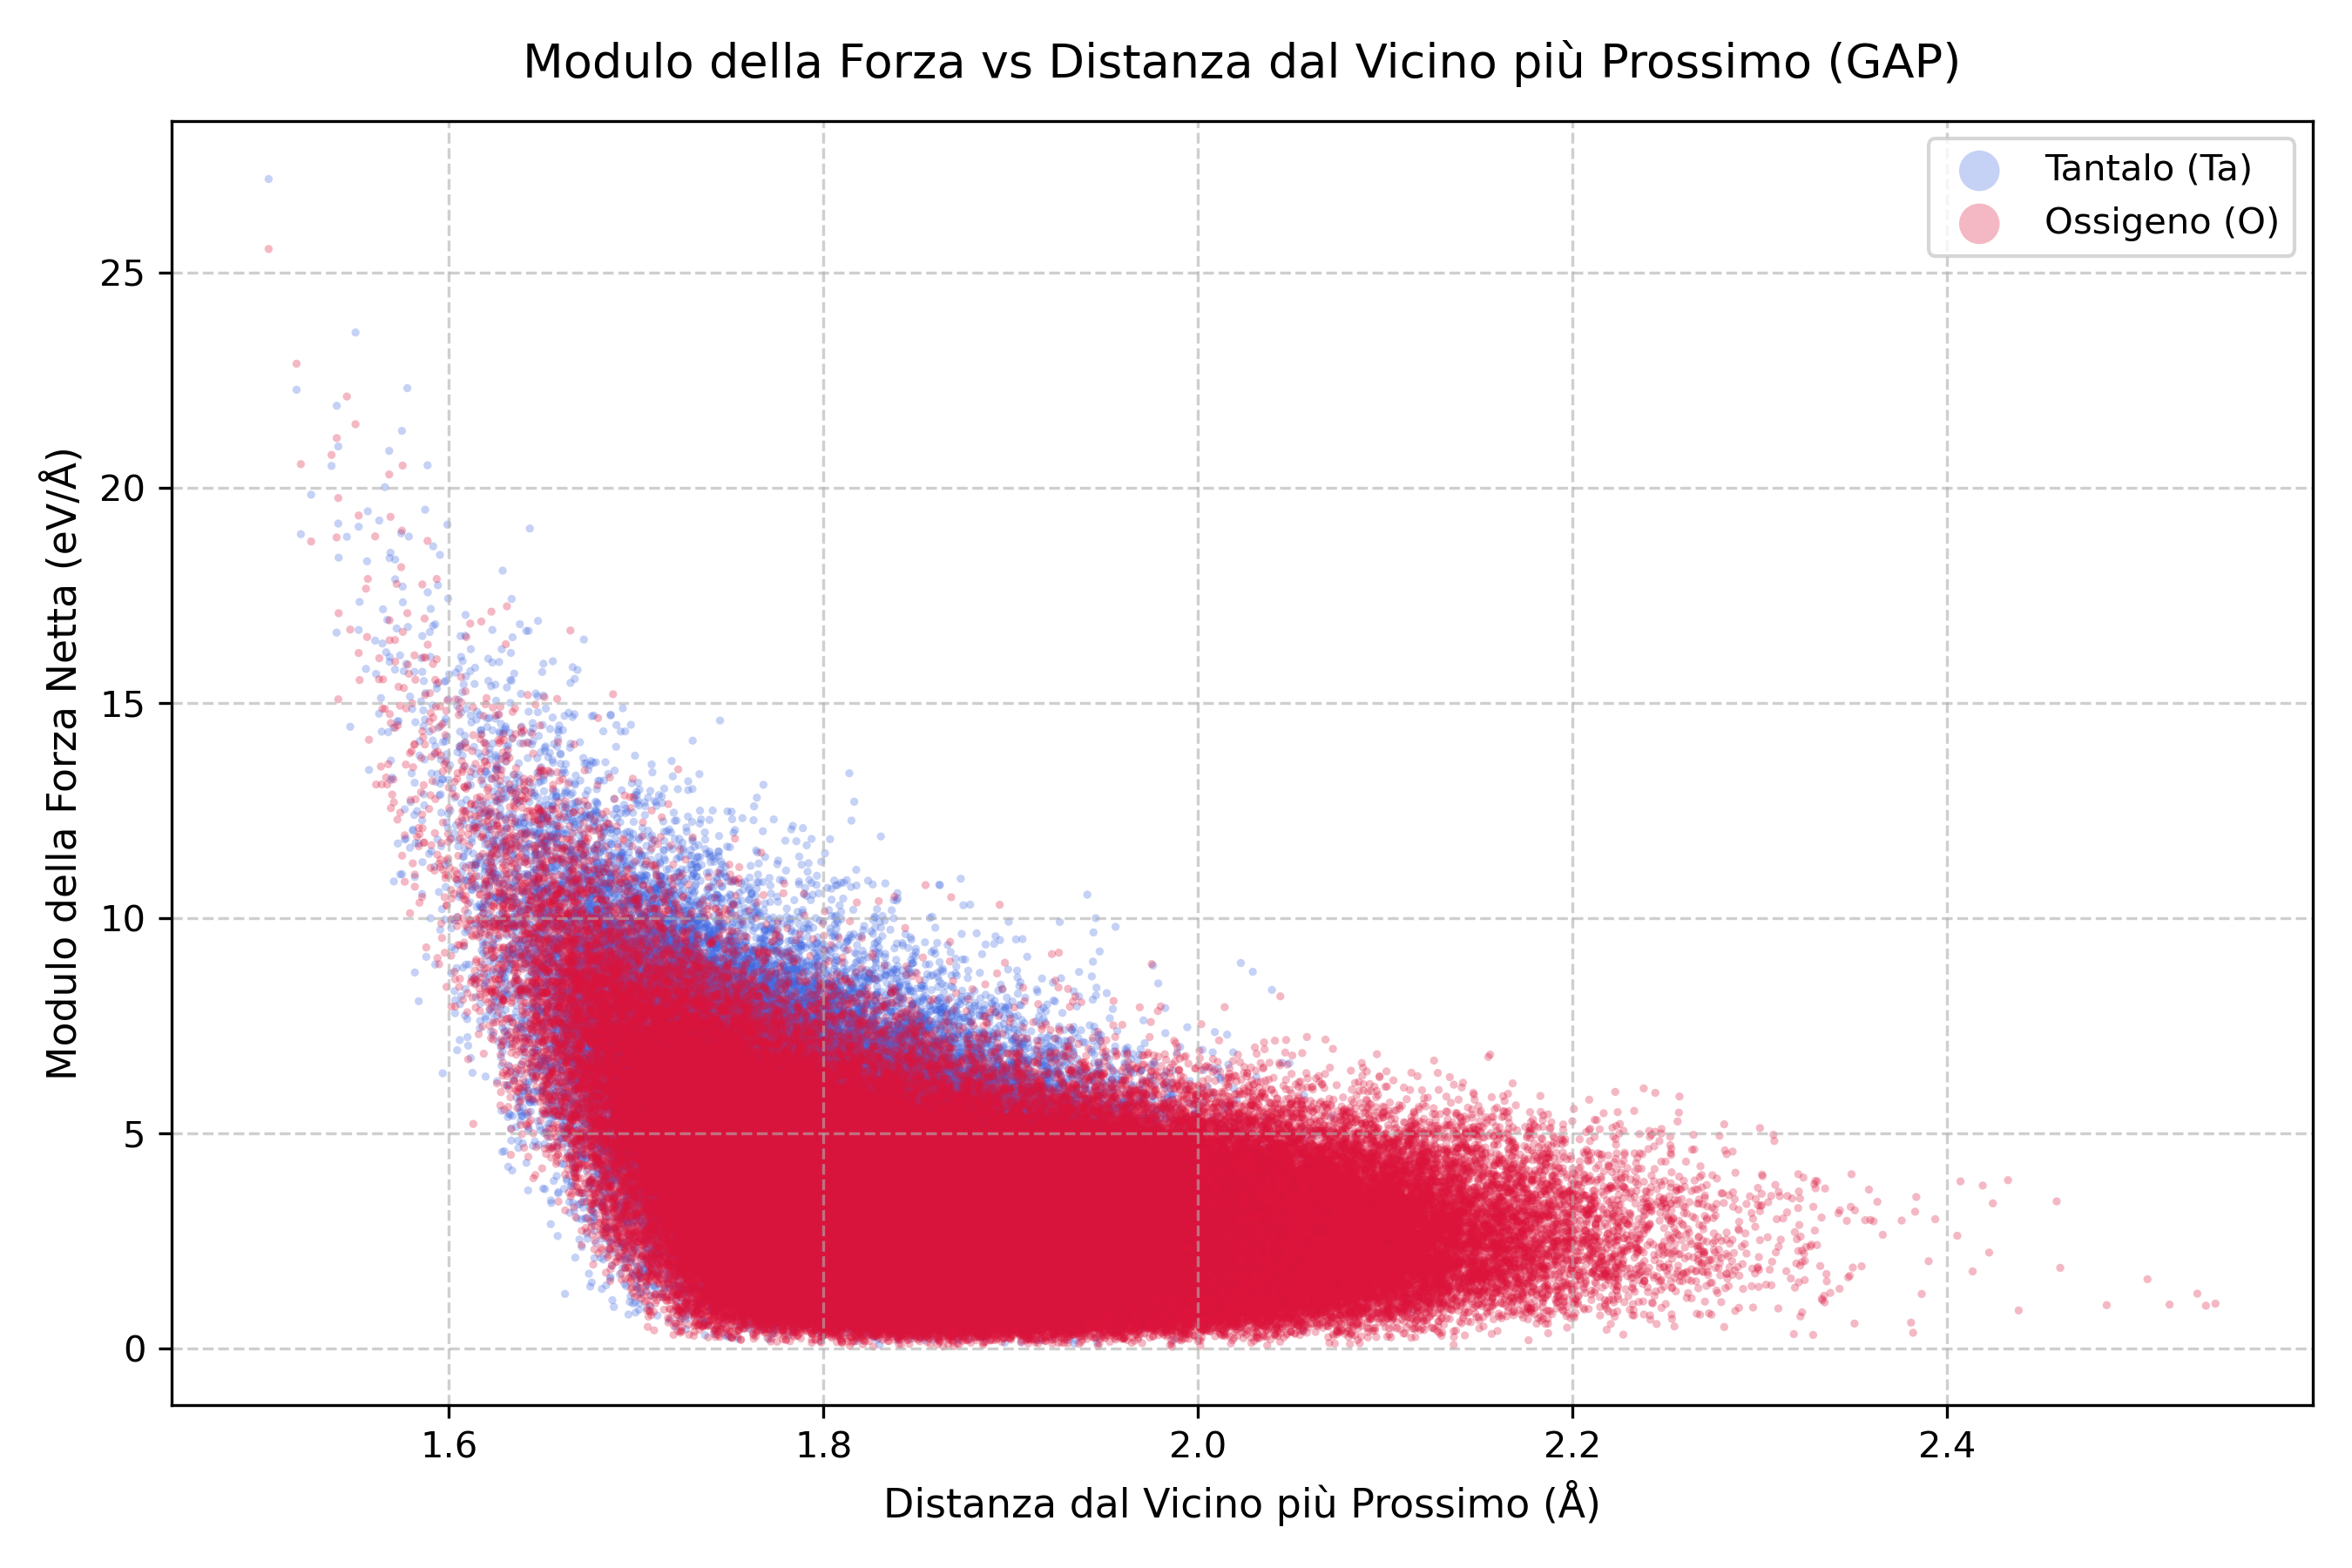
\includegraphics[width=\linewidth]{./img/andamento_forze_totali_distanza_qe_traindata.png}
        \caption{Relazione tra i valori di forza e distanza tra i primi vicini per il set di dati di training}
    \end{subfigure}

    \caption{Distanze e relazione forze distanze per il set di dati di training prodotto con quantum espresso.}
    \label{fig:confronto_forze_distanze_qe_traindata}
\end{figure}
}

quello che notiamo immediatamente, dopo la limitatezza dei valori delle forze, è come la distanza tra i primi vicini assume valori tutti superiori agli $1.5$\AA, inoltre vediamo, che come ci si aspetterebbe, i valori delle forze aumentano alla diminuzione della distanza.


\section{Simulazione con ZBL}

I risultati della sezione precedente sono il principale motivo per il quale andiamo ad addizionare un potenziale repulsivo come lo ZBL.

Anche in questo caso sono stati svolti diversi test, cambiando di volta in volta diversi parametri, non riteniamo necessario riportare tutti questi risultati, inseriamo solo uno di questi, dove l'unica modifica rispetto ai casi precedeti è un timestep di $1$fs.

I parametri per i raggi che abbiamo utilizzato sono dati dal seguente ragionamento, per il $r_{outer} = 1.5$\AA abbiamo deciso di impostare un valore prossimo ai minimi ragistrati nelle configurazioni di training, in questo modo volevamo evitare che lo ZBL si sovrapponesse alle previsioni del GAP. Per quanto riguarda il valore di $r_{inner} = 0.5$\AA abbiamo inserito un valore al quale gli atomi sarebbero sovrapposti e quindi, anche se potrebbe essere alzato, un limite inferiore che dovrebbe essere invalicabile, come si vedrà questo non avviene.

Riportiamo per prima cosa i valori di energia e temperatura

\begin{figure}[h!]
    \centering
    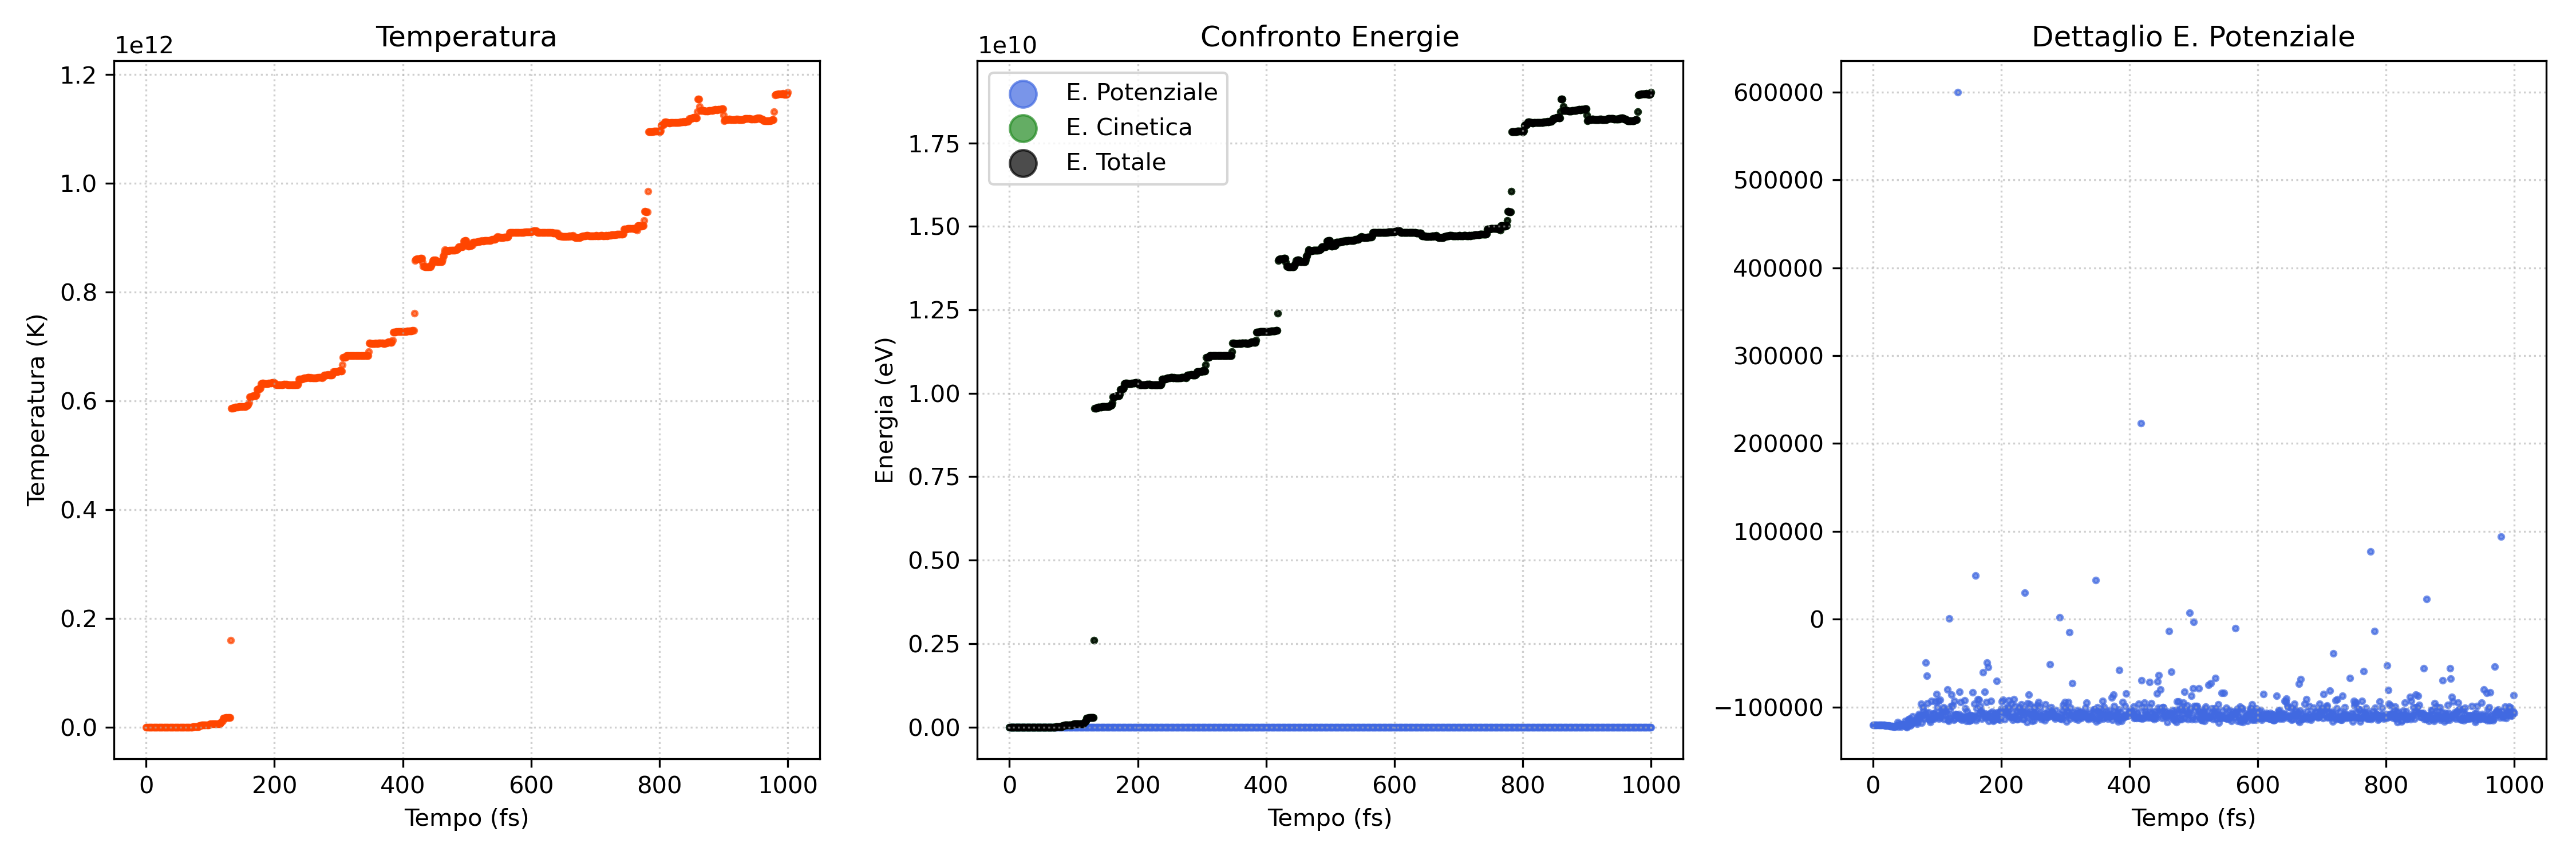
\includegraphics[scale=0.4]{./img/andamento_energia_zbl.png}
    \caption{Grafico dell'andamento temporale per i valori di energia e temperatura, potenziale GAP + ZBL}
    \label{fig:andamento_energia_zbl}
\end{figure}

possiamo vedere come anche in questo caso gli andamenti visti in precedenza si mantengono.

Guardiamo adesso direttamente la relazione tra forze e distanze:

{
\begin{figure}[ht]
    \centering

    \begin{subfigure}{0.48\textwidth}
        \centering
        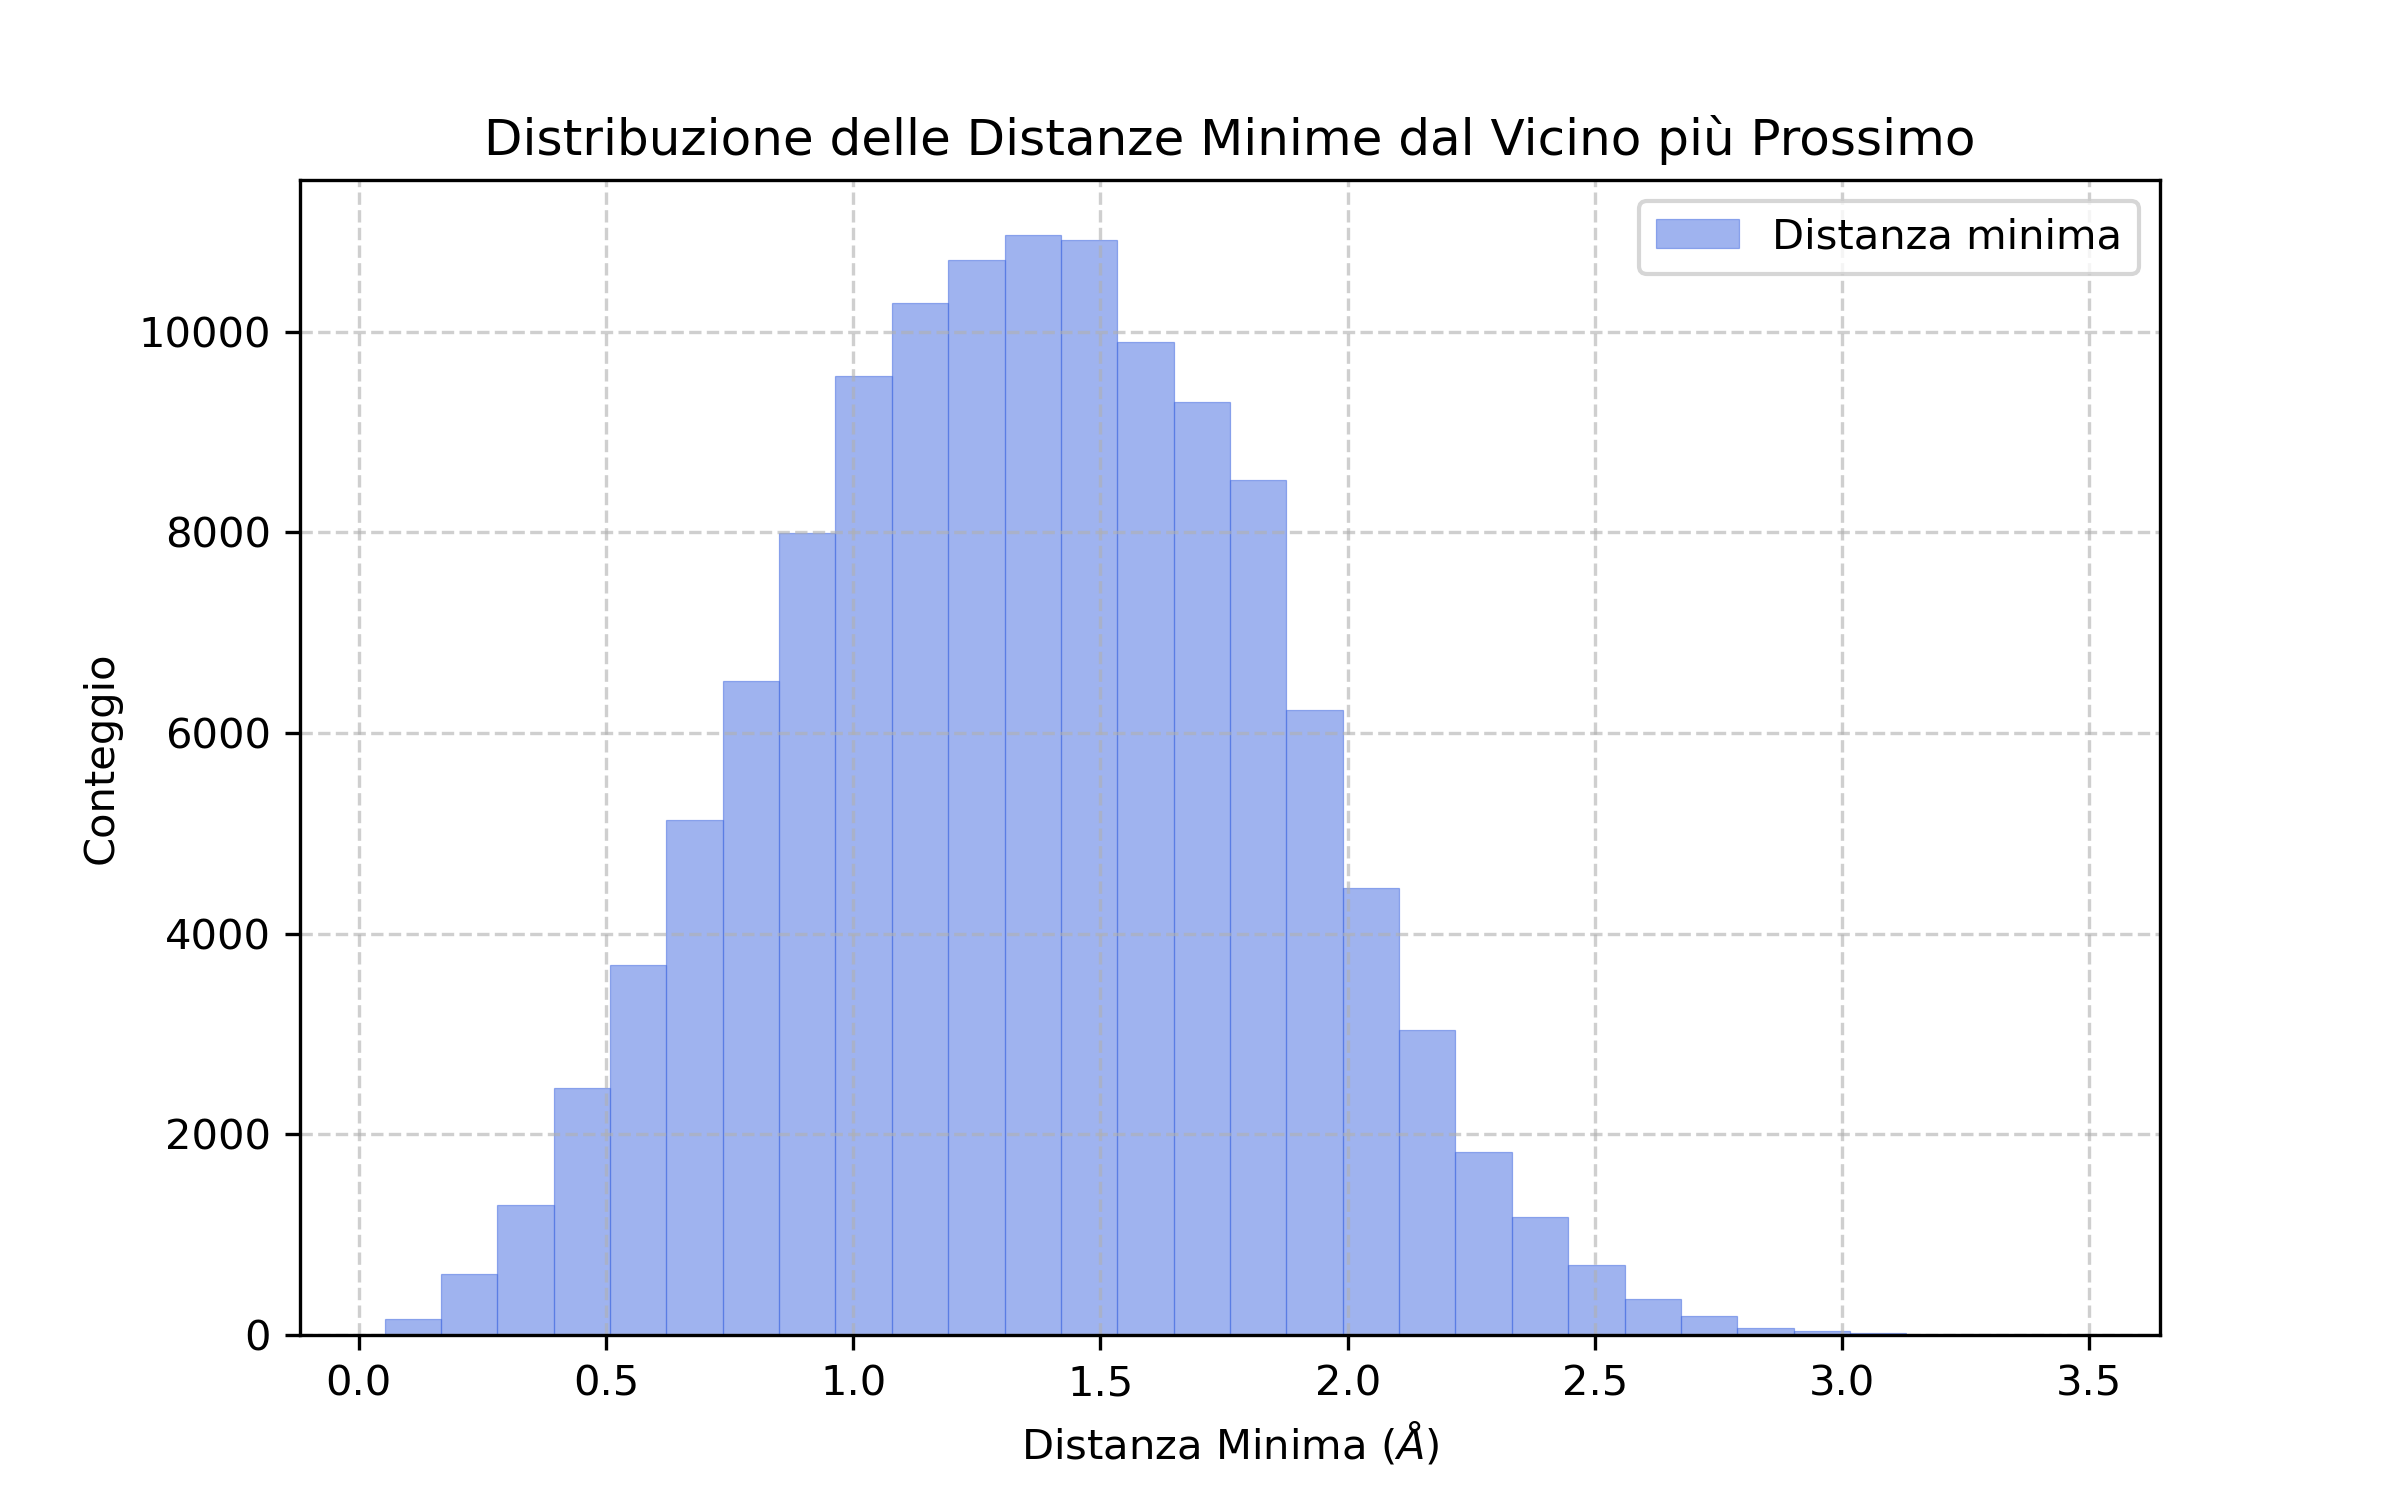
\includegraphics[width=\linewidth]{./img/histo_distanze_zbl.png}
        \caption{Istogramma dei valori di distanza tra i primi vicini per il potenziale GAP + ZBL}
    \end{subfigure}
    \hfill
    \begin{subfigure}{0.48\textwidth}
        \centering
        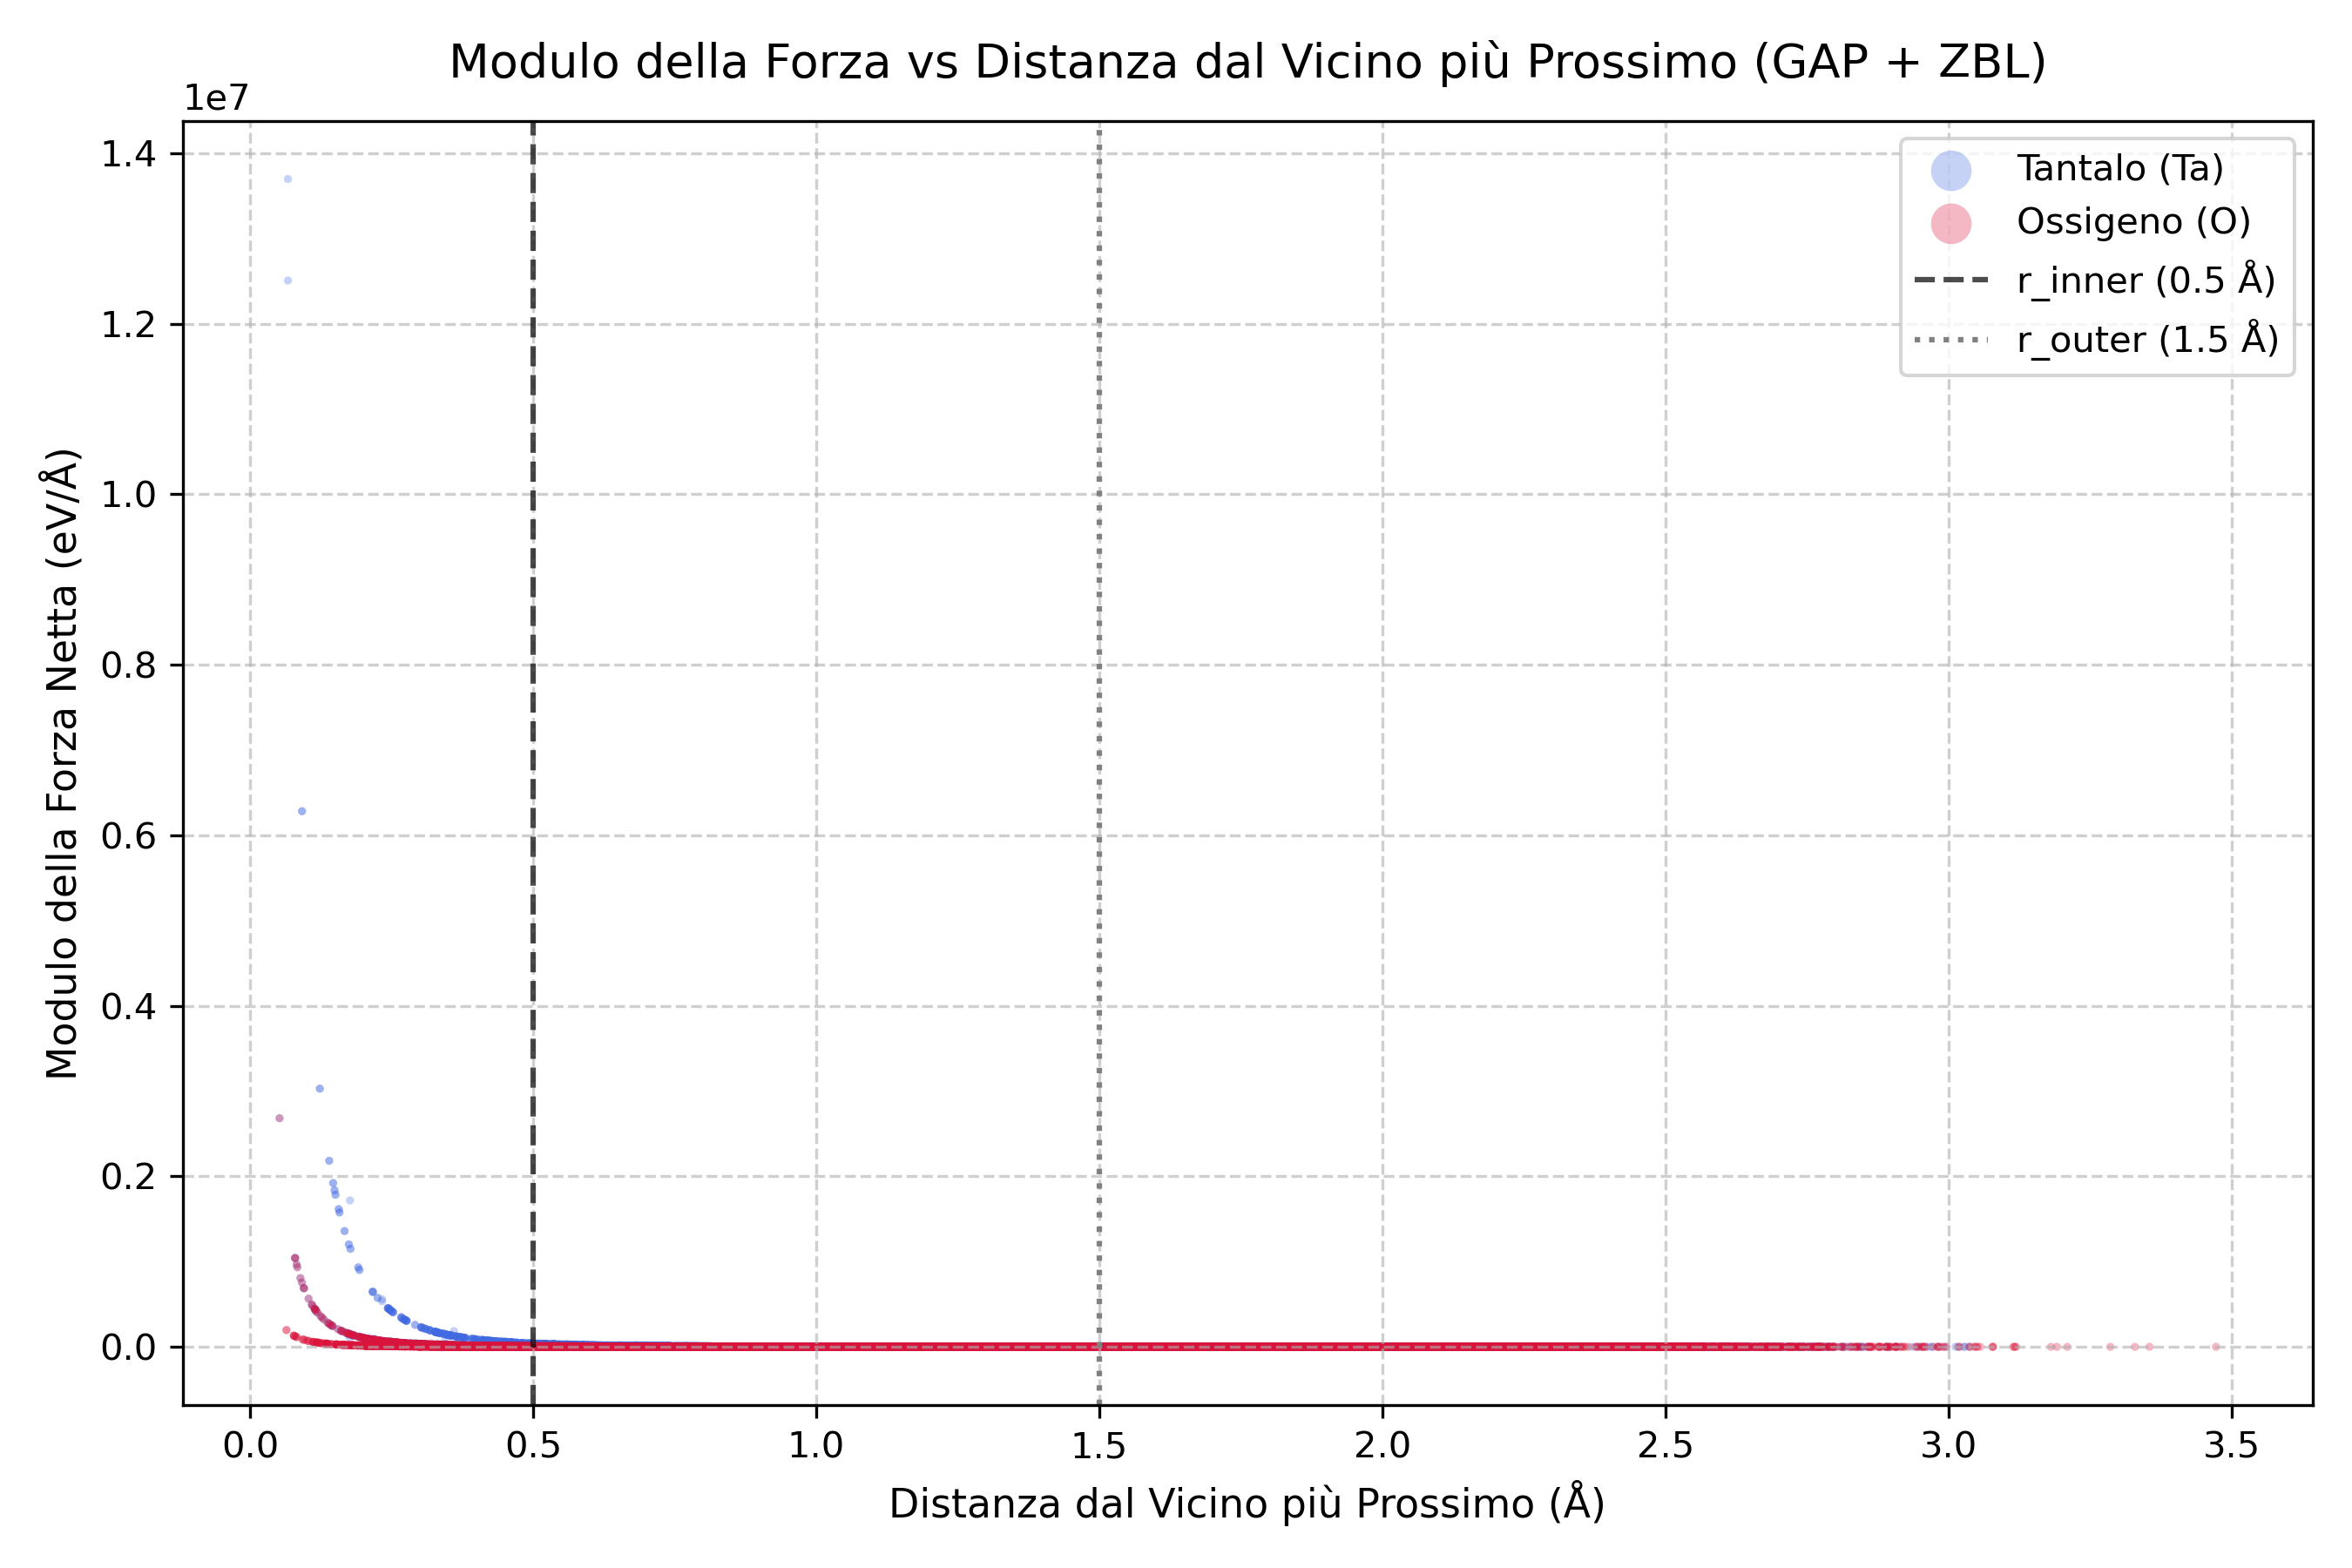
\includegraphics[width=\linewidth]{./img/andamento_forze_totali_distanza_zbl.png}
        \caption{Relazione tra i valori di forza e distanza tra i primi vicini per il potenziale GAP + ZBL}
    \end{subfigure}

    \caption{Distanze e relazione forze distanze per il potenziale GAP + ZBL.}
    \label{fig:confronto_forze_distanze_qe_traindata}
\end{figure}
}

in questo caso è anche utile guardare al confronto tra i due contributi di forza

\begin{figure}[h]
    \centering
    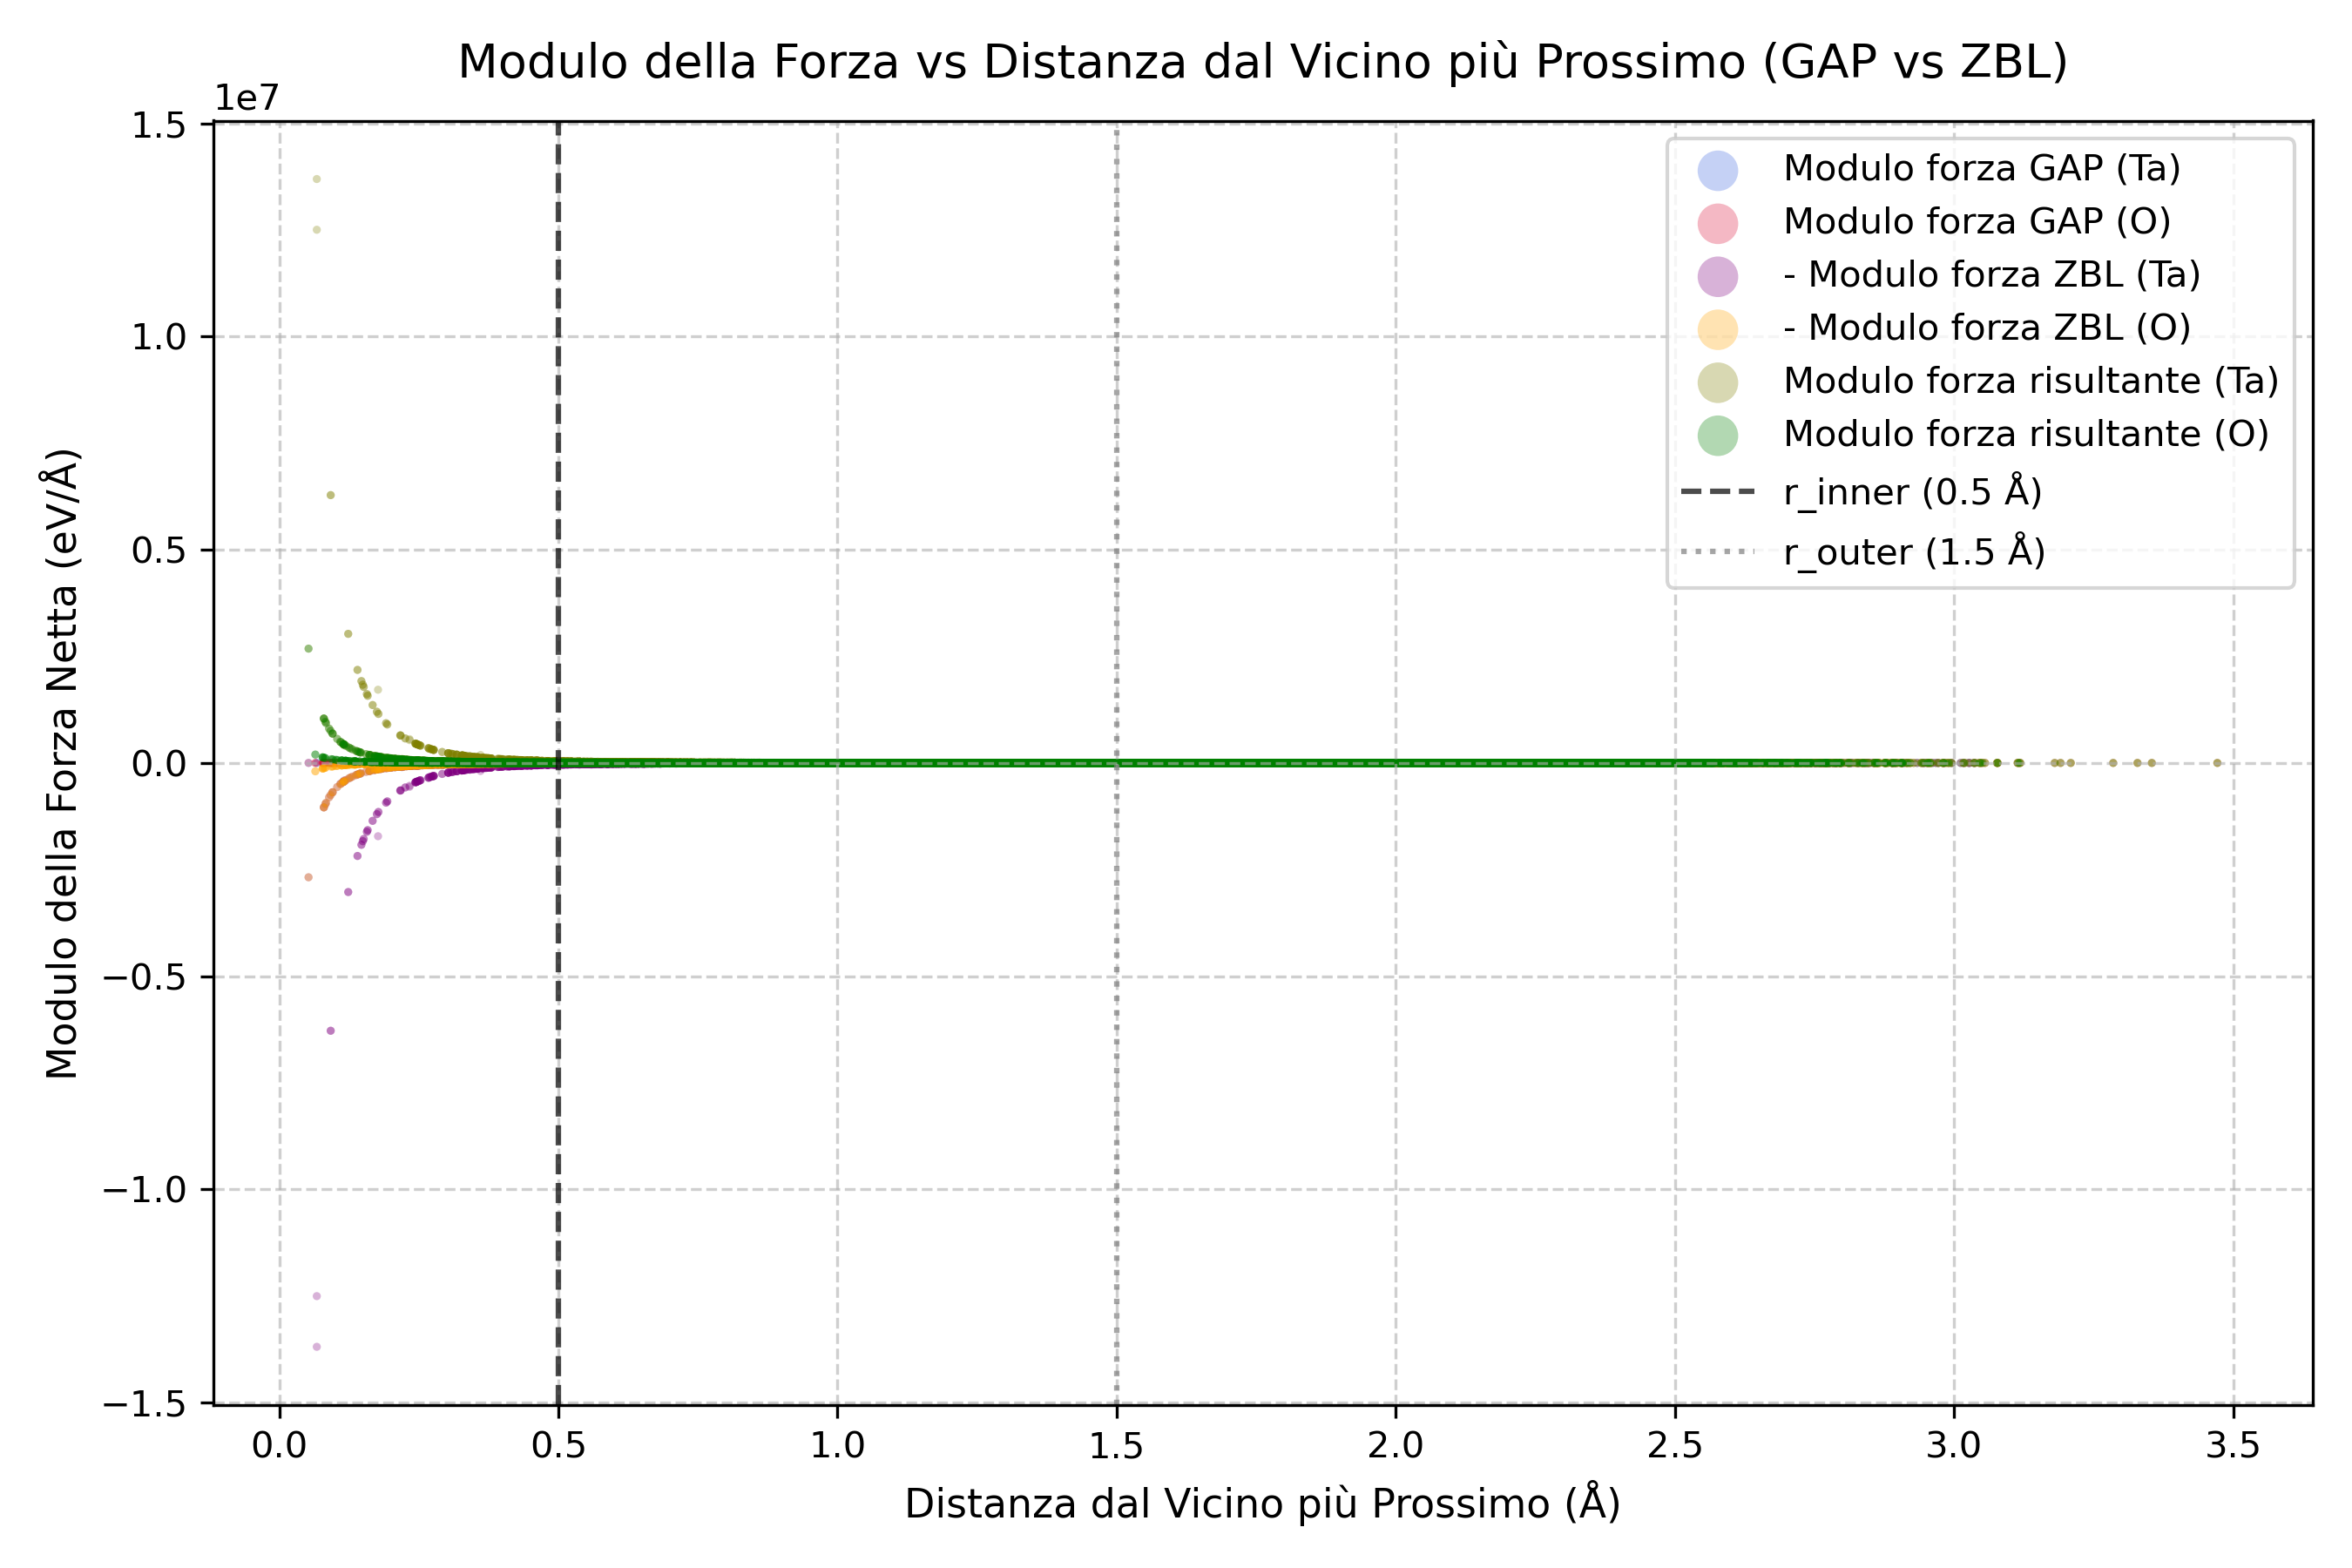
\includegraphics[scale=0.4]{./img/confronto_forze_vs_distanza_minima_zbl.png}
    \caption{Grafico del confronto tra i contributi di forza di GAP e di ZBL}
    \label{fig:confronto_forze_vs_distanza_minima_zbl}
\end{figure}

possiamo notare come i valori di distanza tra i primi vicini arrivino comunque sotto la soglia imposta come minima. Proporniamo come spiegazione di questo fenomeno il fatto che la correzione dello ZBL non sia adeguata a compensare i valori prodotti dal potenziale GAP, essendo questi molto distanti dalle configurazioni di training. Inoltre vogliamo far notare come i moduli delle forze a distanze piccoli siano dati quasi totalmente dalla repulsione prodotta dallo ZBL, questo ci permette di confermare il suo comportamento adeguato, in conclusione non è immediatamente chiaro il motivo per il quale questa correzione non porti a risulati più in linea con le previsioni fatte.

\section{Simulazione con metodo Montecarlo}



